% Endo-HJEPA manuscript — Medical Image Analysis (Elsevier elsarticle).
% Compile: pdflatex endohjepa && bibtex endohjepa && pdflatex endohjepa (x2)
\documentclass[preprint,12pt]{elsarticle}

\usepackage[margin=1in]{geometry}
\usepackage{amsmath,amssymb,bm}
\usepackage{graphicx}
\usepackage{booktabs}
\usepackage{multirow}
\usepackage{array}
\usepackage{algorithm}
\usepackage{algorithmic}
\usepackage{lineno}
\usepackage{hyperref}
\usepackage{xcolor}
\usepackage{placeins}
\graphicspath{{figures/}{./}}
\renewcommand{\topfraction}{0.92}
\renewcommand{\bottomfraction}{0.80}
\renewcommand{\textfraction}{0.08}
\renewcommand{\floatpagefraction}{0.76}
\setcounter{topnumber}{4}
\setcounter{totalnumber}{6}
\newcolumntype{L}[1]{>{\raggedright\arraybackslash}p{#1}}

\journal{Medical Image Analysis}

\begin{document}

\begin{frontmatter}

\title{Endo-HJEPA: Multi-Domain Latent Forecasting with Audited SE(3)-Conditioned Dynamics for Endoscopic Video}

\author[haut]{Ranyang Li\corref{cor1}}
\ead{lry@haut.edu.cn}
\author[hpp]{Nan Wei}
\author[buaa]{Zhipeng Lin}
\author[haut]{Wufeng Liu}
\author[haut]{Chao Fan}
\author[haut]{Xiaodong Guo}
\cortext[cor1]{Corresponding author.}

\address[haut]{School of Artificial Intelligence and Big Data, Henan University of Technology, Zhengzhou 450001, China}
\address[hpp]{Henan Provincial People's Hospital, Zhengzhou 450003, China}
\address[buaa]{School of Computer Science and Engineering, Beihang University, Beijing 100191, China}

\begin{abstract}
Anticipatory assistance in endoscopy requires both forecasting visual dynamics
and testing whether predicted futures respond to measured camera motion.
Prior work rarely separates latent forecast quality from physical action
sensitivity. Endo-HJEPA uses a frozen Video Joint-Embedding Predictive
Architecture~2 large Vision Transformer (V-JEPA~2 ViT-L) across laparoscopic,
gastrointestinal and bronchoscopic video, with a domain-conditioned causal
residual forecaster and a separate
deterministic block-causal branch conditioned on camera-frame special
Euclidean group (SE(3)) increments. Forecast splits are sequence-grouped;
evaluation includes a past-only encoder analysis and two negative-action
protocols. In the
strictly past-only run, mean latent forecast cosine over steps 1--4 is 0.9578,
compared with 0.9102 for its matched persistence baseline. On a separate
750-clip validation cache encoded bidirectionally within each clip, after 6,000
training clips, values are 0.978 for the forecaster,
0.916 for persistence, 0.974 for a gated recurrent unit (GRU) and 0.971 for a
custom Mamba-inspired gated recurrence. On 958 overlapping
windows from four SCARED audit sequences, recorded actions beat a deranged
batch permutation in 88.5\% of windows; a distinct same-sequence bank yields
92.2\% pair wins and 66.4\% all-negative wins. These action results are
audit-selected rather than an independent case-level test. Correcting the
near-wall label timing gives area under the receiver-operating characteristic
curve (AUC) 0.523, so calibrated risk is not established.
The results support multi-domain latent forecasting and
SE(3)-conditioned association under an executable audit, while navigation,
collision warning and clinical efficacy remain outside the claims.
\end{abstract}

\begin{keyword}
world model \sep joint-embedding predictive architecture \sep endoscopy \sep representation learning \sep SE(3)-conditioned prediction \sep evaluation auditing
\end{keyword}

\end{frontmatter}

\linenumbers

\section{Introduction}
\label{sec:intro}

Minimally invasive diagnosis and therapy use visually distinct acquisition
routes: laparoscopes observe the abdominal workspace, gastrointestinal
endoscopes traverse a lumen, and bronchoscopes navigate the airway. In each
setting the camera moves under constrained access while tissue, instruments
and illumination change over time. Anticipating these changes could support
future loss-of-view warning, camera-handling assessment and navigation
research, but present-state recognition alone does not provide a dynamics
model.

Recent surgical video models have begun to predict future pixels or latent
features. Two questions must nevertheless be separated. First, can one model
forecast useful video representations across the three domains? Second, when
metric camera motion is available, is the forecast measurably conditioned on
that motion? The second question cannot be answered by forecast accuracy
alone: observational actions can be ignored, misaligned or confounded with
state. This paper therefore evaluates latent forecasting first and then audits
an SE(3)-conditioned branch under explicit pose and depth signals. The resulting
evidence concerns offline prediction and association, not action execution.

A world model for endoscopy faces a specific asymmetry.
The \emph{structure} of endoscopic video (tissue layout, camera motion and
instrument trajectories) often evolves smoothly over short intervals.
The \emph{appearance} (specular highlights, fluid, smoke, mucosal micro-texture, peristalsis) is high-entropy and largely unpredictable.
The dominant world-model paradigm, pixel generation (diffusion world-action models, Genie-style token video), must also represent this unpredictable appearance.
This can spend model capacity on glare and fluid while tying evaluation to pixel metrics that may be weakly related to the quantities needed for planning.
Joint-embedding predictive architectures (JEPA) offer the alternative adopted
here: predict in a learned representation space that can suppress
unpredictable appearance. Whether those representations carry action-relevant
information is then tested rather than assumed.

\paragraph{Design rationale}
If a frame is written as structure plus appearance, any pixel predictor is lower-bounded by the appearance dispersion, regardless of how well structure is modelled (Section~\ref{sec:theory}).
A representation that is sufficient for structure and invariant to appearance
has no such additive appearance term under the assumptions of
Section~\ref{sec:theory}. This motivates latent prediction without a pixel
decoder. It does not make a latent state physically controllable; the separate
SE(3) audit addresses that question.

\paragraph{Unresolved evaluation problems}
Despite rapid progress in surgical video understanding, four gaps remain.
\textbf{(i) Domain fragmentation.}
Laparoscopic, gastrointestinal and bronchoscopic video are usually evaluated
separately, leaving the value and limits of a shared dynamics model unclear.
\textbf{(ii) Pixel-generation mismatch.}
World models tailored to surgery are predominantly pixel-generative, spending
capacity on the appearance residual that endoscopy makes unpredictable.
\textbf{(iii) Inconsistent forecast protocols.}
Random clip partitions, encoder access to future frames and different
validation caches can produce optimistic or incomparable forecast values.
\textbf{(iv) Untested physical grounding.}
Latent reach or energy scores do not by themselves establish sensitivity to
measured camera motion. An implementation audit of a legacy development
variant found an unexecuted encoder and optimistic planning scores; a separate
temporal-context audit found that a bidirectional video cache let history
tokens contain future-frame context. SE(3)-conditioned
association must therefore be measured
against metric motion and depth, under video-level non-overlap splits and
explicit temporal-context audits, not inferred from forecast accuracy.

\paragraph{Our approach}
We instantiate this idea in \textbf{Endo-HJEPA} (Figure~\ref{fig:pipeline}).
The ``H'' denotes the implemented hierarchical temporal heads (L1 and L2);
because no matched hierarchy ablation is available, it is an architectural
name rather than a claim of demonstrated hierarchical benefit.
A shared frozen V-JEPA~2 ViT-L encoder maps clips from all three domains to dense tokens.
The reported forecast model is a domain-conditioned residual causal L1
predictor. A coarse L2 head is implemented as a temporally pooled mid-horizon
module; we do not report a matched L1-versus-L1+L2 gain study, so headline
forecast evidence is L1-only.
For action-conditioned evaluation, a separate block-causal branch consumes
continuous camera-frame SE(3) increments aligned to SCARED tubelets. A
factorised adapter, probabilistic dynamics and a near-wall head are explored as
auxiliary modules; none is required for the reported action-preference result,
and near-wall risk does not generalise across cases.
The encoder is frozen by default so that every dynamics ablation shares identical latents; an optional last-block adaptation is evaluated only on recognition probes.
No pixel decoder is trained.
The evidence is scoped as follows: forecast and scale are measured on a
6{,}000-clip causal-L1 protocol; the physical branch is trained and selected
under case-level development splits and reported on a previously contacted,
audit-selected SCARED partition; recognition uses frozen V-JEPA~2 on the
official CholecT50 split.
Results from these protocols are reported separately.

\begin{figure}[t]
\centering
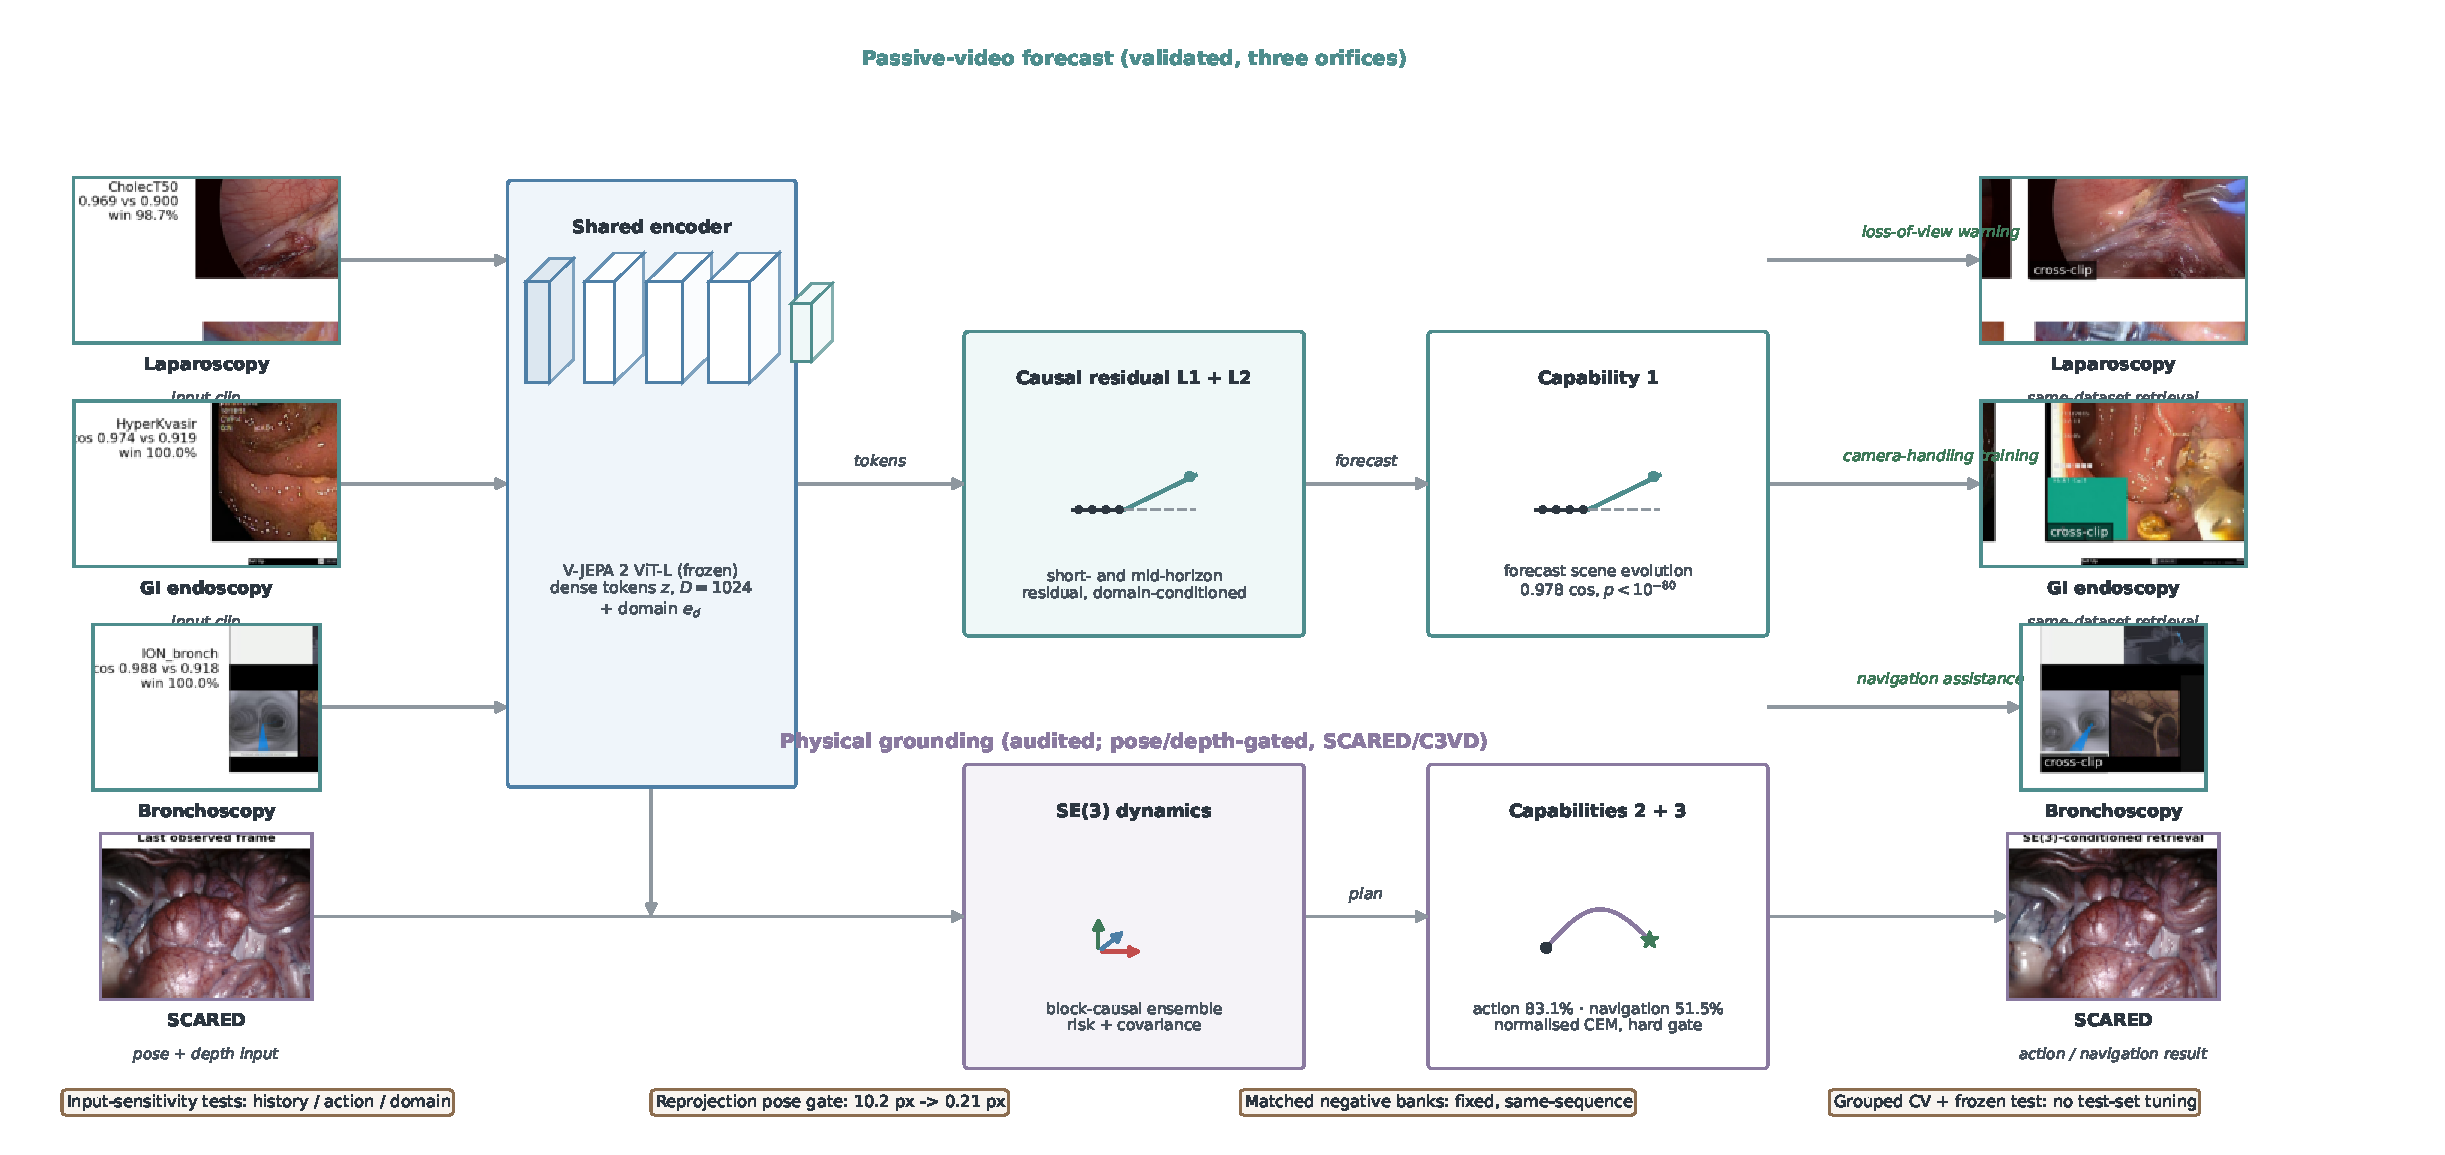
\includegraphics[width=\textwidth]{figure1_pipeline.pdf}
\caption{Endo-HJEPA overview. Lane~A: complete displayed validation frames
from laparoscopy (CholecT50), GI endoscopy (Kvasir-Capsule) and bronchoscopy
(ION, whose native format is a navigation-console capture) enter the shared
frozen V-JEPA~2 encoder, drawn here as its own layer stack, and the causal
forecaster returns the nearest-latent frame from a \emph{different clip of the
same dataset}, so every input row has its own matched output row. The predictor
column exposes the two temporal scales separately, pooled causal L1 and pooled
coarse L2, and the capability column carries the measured forecast scaling
curve of Figure~\ref{fig:forecast} against the persistence baseline, with the
13,552-clip point drawn open because it uses a different validation cache. The
qualitative retrieval rows use this 13,552-clip checkpoint; the $0.978$ scale
inset value remains the matched 6,000-clip result. Lane~B
turns calibrated SCARED pose into window-end-aligned SE(3) twists and combines
them with past-only tokens rebuilt using the same frozen encoder weights. Its
deterministic block-causal dynamics report the
action-evaluation and forced-future oracle-retrieval diagnostic. The risk head and
candidate filter are unused exploratory modules: corrected-label
near-wall AUC is $0.523$, below the $0.75$ gate, and neither is active in the
reported proxy. Italic green labels name proposed
research pathways, not evaluated clinical applications. The bottom strip lists
four correctness-audit checks. All displayed output frames are
nearest-neighbour retrievals rather than generated pixels. Lane~A thumbnails
are selected for high tissue
visibility among clips whose forecast beats persistence; Lane~B uses an
audit-partition SCARED retrieval example. Both are illustrative examples
selected by disclosed rules; neither is a random sample or a basis for
quantitative comparison.}
\label{fig:pipeline}
\end{figure}

\paragraph{Contributions}
\begin{enumerate}
  \item \textbf{A shared latent forecaster across endoscopic domains.}
  We instantiate residual short-horizon dynamics on the official V-JEPA~2
  ViT-L encoder across laparoscopic, GI and bronchoscopic video with one
  domain-conditioned model. A coarse L2 head is implemented, but the reported
  forecast evidence is L1-only because no matched L1-versus-L1+L2 comparison is
  available.
  \item \textbf{A causal-autoregressive latent forecaster.}
  A decoder-style residual Transformer improves mean steps-1--4 cosine over
  persistence, GRU and a custom Mamba-inspired recurrence on the same
  validation cache. A separate
  past-only encoder run quantifies the effect of temporal context.
  \item \textbf{An audited SE(3)-conditioned evaluation path.}
  We exclude invalid discrete-MPC evidence and build a corrected continuous
  SE(3) branch whose deranged-batch action-preference result is 88.5\% on 958
  overlapping SCARED audit windows. The contribution includes
  executable audit:
  input-sensitivity tests, a C3VD depth-warp diagnostic and two explicitly
  defined negative protocols. It supports conditioned association, not causal
  intervention, safety or robot control.
  \item \textbf{A transparent, per-dataset evaluation protocol.}
  Video-level non-overlap splits, domain-balanced sampling, per-dataset
  forecast decomposition, temporal-context audits, reproducible external
  baselines and paired tests released as executable code.
\end{enumerate}

\paragraph{Evidence and scope}
The 19-corpus census contains 1{,}707 local manifest units; the 13,552-clip forecast cache
contains 11 datasets. On the matched 6,000-clip protocol, the causal forecaster
reaches 0.978 mean cosine over steps 1--4 against 0.916 persistence, 0.974 GRU
and 0.971 for the custom gated recurrence, with monotone scaling to 6,000
clips. The 13,552-clip point
uses a different validation cache and is not used to infer a plateau.
Two characterised negative results complete the
picture: self-supervised latent actions are not semantically or physically
grounded without encoder-level supervision, and zero-shot cross-domain
transfer improves partially with a 32-shot domain token but remains below
persistence. This motivates, but does not establish the superiority of,
unified multi-domain training.
We do \emph{not} claim the first surgical world model, pixel-level video
generation, robot-executed planning, uniform recognition SOTA, or any clinical
efficacy endpoint.

\paragraph{Significance}
Endo-HJEPA studies anticipatory representation modelling beyond present-state
recognition.
The motivation is anticipation under data scarcity across endoscopic domains. The
current evidence is offline representation prediction and SE(3)-conditioned
association; it does not validate collision warning, calibrated physical risk
or clinical benefit.

\section{Related work}
We position Endo-HJEPA along five axes: the world-model lineage it builds on, the surgical/endoscopic representation learning it extends, the surgical world models it differs from, the general video/image backbones we benchmark against, and the endoscopic datasets that anchor our evaluation.

\subsection{World models and joint-embedding prediction}
The idea of a learned world model for prediction and planning originates with
Ha and Schmidhuber's World Models~\cite{ha2018worldmodels} and the PlaNet
latent-dynamics planner~\cite{hafner2019planet}, and was scaled to diverse
control domains by Dreamer~\cite{hafner2023dreamer}. Energy-based
formulations~\cite{lecun2006ebm} provide a general framework for scoring state
compatibility. JEPA~\cite{lecun2022path} instead predicts in representation
space; I-JEPA~\cite{assran2023ijepa} applies the principle to images,
V-JEPA~\cite{bardes2024vjepa} to video, and V-JEPA~2 and its action-conditioned
variant extend it to large-scale video understanding and robot
planning~\cite{assran2025vjepa2}. Generative interactive environments such as
Genie~\cite{genie2024} model pixels. These systems establish the general
world-model design space but do not evaluate camera-frame SE(3)-conditioned
dynamics in endoscopic video.

\subsection{Self-supervised surgical and endoscopic video representation}
Self-supervised pretraining has become common in surgical video.
SurgRec-JEPA~\cite{surgrecjepa} and JHU-VPT~\cite{jhuvpt} report strong
downstream transfer, while Endo-FM~\cite{endofoundation} scales pretraining on
endoscopic corpora and SurgMotion~\cite{surgmotion} develops video-native
surgical representations. SurgRec-JEPA includes a latent predictive objective, so it
is not merely a recognition model; its released backbone is used for
downstream representation learning rather than metric endoscope control.
Endo-HJEPA focuses on the complementary evaluation of multi-domain temporal
forecasting and an explicitly supervised camera-motion interface.

\subsection{Surgical and endoscopic world models}
World models tailored to surgery are emerging. The Surgical Vision World
Model~\cite{svwm} generates pixel-controllable surgical video, and
EndoWAM~\cite{endowam} applies diffusion world-action modelling to endoscopic
navigation. SurgVista~\cite{surgvista} studies long-horizon instrument--tissue
dynamics, while Surg-UniWorld~\cite{surguniworld} studies multimodal control of
surgical video generation. SurgFUTR and SFPBench evaluate labelled future-event
anticipation~\cite{surgfutr}. SurgWMBench evaluates instrument-motion world
models through local transitions, autoregressive rollouts and perturbation
recovery~\cite{surgwmbench}. Dual-endoscope future video prediction is
studied by CrossScope~\cite{crossscope}. These tasks and metrics do not match our
pooled-latent or camera-motion protocols. Our contribution is representation
prediction with an audited SE(3) evaluation path; our experiments test, rather
than assume, whether passive JEPA features support metric action association
or calibrated risk.

\subsection{General video and image representation backbones}
For representation evaluation, we benchmark the evaluated \emph{reproducible}
general-purpose encoders. Video baselines are VideoMAE~\cite{tong2022videomae}
(Kinetics masked autoencoding), TimeSformer~\cite{timesformer} (divided
space-time attention), and ViViT~\cite{vivit} (factorised space-time).
VideoMamba~\cite{videomamba} and Mamba~\cite{mamba} provide state-space-model
(SSM) background. Our lightweight comparator is a custom Mamba-inspired gated
recurrence rather than either reference implementation. Image baselines are the ImageNet-supervised
ViT~\cite{dosovitskiy2021vit} and temporally pooled DINOv2
features~\cite{dinov2}. CholecT50 probes compare representation transfer only;
they do not serve as planning or world-model baselines.

\subsection{Endoscopic datasets and physical supervision signals}
Our corpus census includes Cholec80~\cite{twinanda2017endonet},
CholecT50~\cite{nwoye2022rendezvous,nwoye2022cholectsplit}, EndoVis
2015 instrument tracking and EndoVis 2017/2018 robotic-instrument
segmentation~\cite{bodenstedt2018endovis,endovis2017,endovis2018},
CholecSeg8k~\cite{hong2020cholecseg8k},
Endoscapes~\cite{endoscapes}, HyperKvasir~\cite{borgli2020hyperkvasir},
Kvasir-Capsule~\cite{kvasircapsule}, Kvasir-Instrument~\cite{jha2021kvasirinstrument},
SCARED~\cite{allan2021scared}, C3VD/C3VDv2~\cite{bobrow2023c3vd,golhar2026c3vdv2},
EndoNeRF~\cite{wang2022endonerf},
TrackVes~\cite{trackves2021,penza2018trackves},
Surgical Tattoos in Infrared (STIR)~\cite{stir2024}, SurgT~\cite{cartucho2024surgt}
and the Hamlyn rectified stereo corpus~\cite{recasens2021endodepth}. Their roles differ:
RGB video supports latent forecasting, SCARED poses supervise the action
branch, C3VD supports a convention-specific depth-warp diagnostic, and STIR is
an exploratory deformation extension.

\paragraph{Summary} The field offers strong self-supervised representations,
pixel-generative surgical world models and general video/image backbones.
Endo-HJEPA studies a
representation-prediction design, with an implemented but unablated coarse L2
head, and an explicitly audited SE(3)-conditioned evaluation path; its risk
and control limits are part of the result.

\section{Method}
\label{sec:method}

\paragraph{Core idea}
Endo-HJEPA separates two questions without generating pixels:
(i)~given a history of endoscopic tokens, what is the likely future
representation; and (ii)~given a \emph{measured camera motion}, does a
block-causal predictor use that motion to improve the future latent estimate?
The reported forecast result uses causal L1; L2 is implemented but not
separately evaluated. The second question is conditioned on continuous SE(3),
not an emergent residual code. CEM and near-wall risk are reported only as
diagnostics because neither yields an executed-control result.
Residual anchoring and uncertainty weighting belong to the core pooled model.
Dense variance-invariance-covariance regularisation (VICReg), appearance
weighting and STIR supervision are explicitly
separated below as optional spatial or encoder-adaptation extensions; they are
excluded from the pooled forecast numbers.
Figure~\ref{fig:pipeline} gives the study-level data flow,
Figure~\ref{fig:network} gives the tensor-level model, and
Table~\ref{tab:notation} lists symbols.

\begin{figure}[p]
\centering
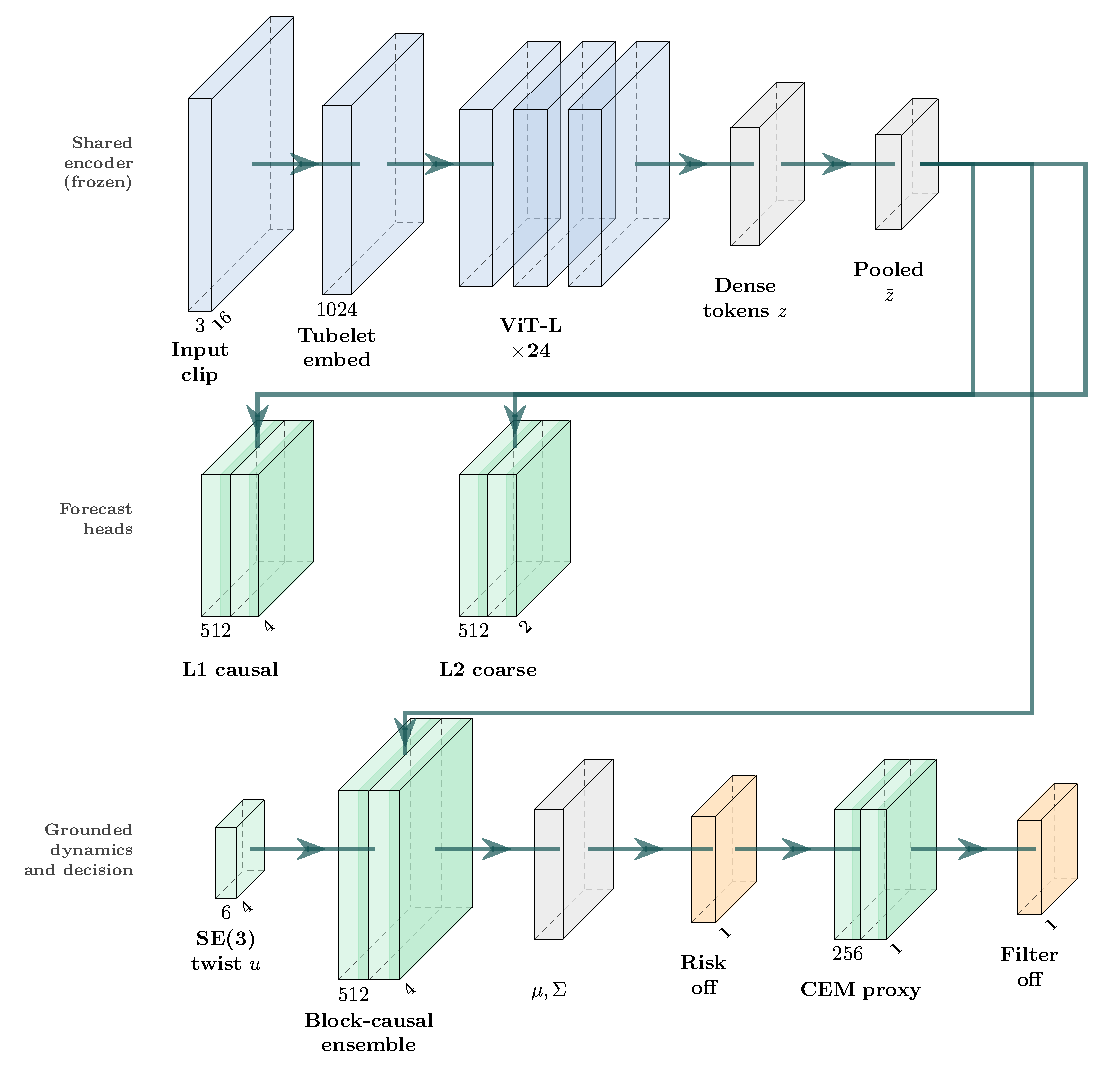
\includegraphics[width=0.92\textwidth]{figure1_network.pdf}
\caption{Detailed network model rendered with PlotNeuralNet, laid out as three
rows. Row~1 is the frozen V-JEPA~2 ViT-L encoder, from the clip through the
tubelet embedding and the 24 space-time blocks to dense tokens, followed by
spatial pooling to $\bar z$. Row~2 is
the forecast branch, with separate causal Level-1 (L1) and coarse Level-2 (L2)
heads trained
against frozen latent targets. Row~3 is the grounded branch,
where the continuous SE(3) twist and a deterministic block-causal predictor
produce the latent rollout used by the cross-entropy method (CEM) diagnostic.
The inactive
risk head and rejection rule are omitted from this active path: the reported
oracle-goal proxy uses a dynamics checkpoint without either module, and
corrected-label near-wall AUC is $0.523$ (fail). Blue denotes the frozen visual
encoder, teal the trained prediction modules and grey the latent tensors. Both
branch rows use the same frozen encoder weights and pooled interface, but the
physical audit uses a separately rebuilt past-only cache. The action branch
uses measured pose where available; no pixel decoder is trained.}
\label{fig:network}
\end{figure}

\begin{table}[t]
\centering
\caption{Principal notation (Section~\ref{sec:method}).}
\label{tab:notation}
\scriptsize
\begin{tabular}{@{}lp{0.68\textwidth}@{}}
\toprule
Symbol & Meaning \\
\midrule
$x_{1:T}$, $d$ & Input clip of $T$ frames; domain $d\in\{\mathrm{laparo},\mathrm{gi},\mathrm{bronch}\}$ \\
$f_\theta$, $z_{1:T'}$ & Frozen encoder; dense tokens $z\in\mathbb{R}^{T'\times N\times D}$ \\
$g_\phi$, $\hat{\bar z}$; $g_\phi^{\mathrm{dense}}$, $\hat z$ & Headline pooled predictor/output; optional dense predictor/output \\
$T',N,D$ & Tubelet steps ($T/2$), spatial tokens ($256$), width ($1024$) \\
$\bar z_t$ & Spatially pooled token $\frac{1}{N}\sum_{n=1}^{N}z_{t,n}\in\mathbb{R}^{D}$ \\
$e_d$ & Learnable domain embedding \\
$B,H,H_{\mathrm{hist}}$ & Batch size, forecast horizon and history (the latter two default to $4$) \\
$\mathbf{T}_t\in\mathrm{SE}(3)$ & Camera-to-world pose at the retained window-end time $t$ \\
$u_t=\log(\mathbf{T}_t^{-1}\mathbf{T}_{t+1})^\vee\in\mathbb{R}^6$ & Measured camera-frame twist $[v_t;\omega_t]$; SCARED uses mm and rad per four native frames; $\vee$ vectorises $\mathfrak{se}(3)$ \\
$\tilde u_t=(u_t-\mu_u)\oslash\sigma_u$ & Per-axis action normalisation fitted on the relevant training split; $\oslash$ is elementwise division \\
$s_t^{g},s_t^{q},s_t^{m},\xi_t$ & Geometry, tool, slow-semantic and nuisance slots (used by auxiliary losses, not inside the current CEM loop) \\
$\bar z^\star$ & Oracle terminal pooled latent used only by the CEM retrieval diagnostic \\
$\bar r_t=\bar z_{t+1}-\bar z_t$; $r_t=z_{t+1}-z_t$ & Pooled residual used by the headline forecaster; dense residual used by the legacy vector-quantisation (VQ) audit \\
$a_t,z^{-}$ & Legacy discrete residual code and rolled negative latent for the energy audit \\
$p_{\mathrm{wall}},\Sigma_{\mathrm{ale}},\Sigma_{\mathrm{epi}}$ & Exploratory near-wall score and aleatoric/epistemic uncertainty \\
$d^{5\%}_t,y_{\mathrm{wall},t}$ & Fifth percentile of valid SCARED depth (mm); binary near-wall label $\mathbf{1}[d^{5\%}_t<34.4\,\mathrm{mm}]$ \\
$M_e,\mu_m,\sigma_m^2$ & Number of ensemble members and member-$m$ Gaussian mean/diagonal variance \\
$s^{\mathrm{plan}}_{bkj},D_s$ & Target coordinate and state width of planner dynamics; the current pooled implementation uses $s^{\mathrm{plan}}=\bar z$ and $D_s=D$ \\
$s_i$ & Learnable log-variance of loss term $i$ \\
$\rho(a,b)$; $\delta$ & Elementwise Smooth-$L_1$ penalty and its transition point ($\delta=1$) \\
$\mu_u,\sigma_u$ & Per-axis mean and standard deviation of actions, fitted on training data only \\
$\mathcal{A}_{\mathrm{pool}}$ & Active pooled losses, a subset of $\{\mathrm{L1},\mathrm{L2}\}$ \\
$\lambda_r,\lambda_u,\lambda_s,\lambda_e$ & Search weights for risk, uncertainty, action smoothness and latent-path smoothness \\
$p_t,M$ & Temporal positional encoding and causal attention mask \\
$w,w_{\min},\beta,m_{\mathrm{inst}}$ & Tubelet weight, floor, mask gain and instrument occupancy \\
\bottomrule
\end{tabular}
\end{table}

\subsection{Problem formulation and assumptions}
\label{sec:formulation}
A clip $x_{1:T}$ from domain $d$ is mapped by a frozen encoder $f_\theta$ to
\begin{equation}
z_{1:T'}=f_\theta(x_{1:T})\in\mathbb{R}^{T'\times N\times D},\qquad T'=T/2,\; N=256,\; D=1024.
\label{eq:encode}
\end{equation}
Headline pooled forecast operates on the spatially pooled token
\begin{equation}
\bar z_t=\frac{1}{N}\sum_{n=1}^{N}z_{t,n}\in\mathbb{R}^{D},
\label{eq:pool}
\end{equation}
averaging over the $N$ spatial sites. The world model is a collection of
predictors $g_\phi$ on $\bar z_t$ (pooled) or $z_{t,n}$ (dense extension) and
never decodes pixels. The passive branch has two temporal scales:
L1 forecasts $\hat{\bar z}_{t+1:t+H}$ on the original latent stream, whereas
L2 forecasts a stride-$2$ temporally pooled stream. These labels denote
temporal levels, not $L_1/L_2$ norms or verified semantic factors. The
reported forecast evidence is L1-only, since no matched
L1-versus-L1{+}L2 ablation is reported. For physical grounding, a low-rank
adapter decomposes $z_t\mapsto(s_t^g,s_t^q,s_t^m,\xi_t)$ for downstream
slot-level analysis and loss construction. The implemented planner rolls the
full pooled latent $\bar z_t$ directly (the factorised adapter is not in the
CEM/MPPI loop), so the continuous search objective is
\begin{equation}
\begin{aligned}
\hat{\tilde u}_{t:t+H-1}
\approx{}&\arg\min_{\tilde u_{t:t+H-1}}\;
\frac{1}{D}\bigl\|\hat{\bar z}_{t+H}(\tilde u_{t:t+H-1})-\bar z^\star\bigr\|_2^2
+\lambda_r\,\frac{1}{H}\sum_{k=0}^{H-1}p_{\mathrm{wall},t+k}\\
&{}+\lambda_u\,\frac{1}{H}\sum_{k=0}^{H-1}
(\overline{\operatorname{Var}}_{\mathrm{ale},t+k}
+\overline{\operatorname{Var}}_{\mathrm{epi},t+k})
\\
&{}+\lambda_s\,\frac{1}{6(H-1)}\sum_{k=1}^{H-1}
\|\tilde u_{t+k}-\tilde u_{t+k-1}\|_2^2
\\
&{}+\lambda_e\,\overline{\Delta^2}_{\mathrm{path}} .
\end{aligned}
\label{eq:mpc}
\end{equation}
The minimisation variable is the normalised action $\tilde u$; the reported
search clips each coordinate to $[-2.5,2.5]$. Its wrapper maps candidates back
to raw $u$ before invoking the deterministic model, whose input layer applies
the same training-set normalisation. This round trip is algebraically
equivalent to supplying $\tilde u$ once and keeps the model's public interface
in physical units. Here
$\overline{\operatorname{Var}}$ denotes the mean over the $D$ latent
dimensions (not the trace), and
$\overline{\Delta^2}_{\mathrm{path}}$ is the mean squared change between
successive predicted latents, including the final history latent as its first
anchor. It is a smoothness surrogate, not the legacy discrete energy
$E(z,a,z')$. The implementation averages risk and uncertainty over the
horizon, as written above. Candidate thresholds can reject high-risk or
high-uncertainty sequences. The reported oracle-goal proxy uses a deterministic
checkpoint, so its risk and uncertainty terms are identically zero; only goal
matching, action smoothness and latent-path smoothness contribute. It therefore
does not evaluate the rejection filter. For $H=1$, the action-smoothness term
in~\eqref{eq:mpc} is defined as zero.

\emph{Assumptions.}
(i)~Endoscopic dynamics are approximately Markovian in the learned latent space at the tubelet timescale.
(ii)~The frozen V-JEPA~2 encoder is assumed to suppress some appearance
nuisance; the pixel-generation contrast in \S\ref{sec:rq1} motivates, but does
not prove, this representation-level assumption.
(iii)~The three domains may share short-timescale visual dynamics while still
requiring explicit domain conditioning; Section~\ref{sec:rq4} tests this
hypothesis.

\subsection{Shared encoder and optional endoscopic token weighting}
The encoder is the publicly released V-JEPA~2 ViT-L model (patch $16$, tubelet
$2$, input $256^2$), kept frozen by default.
For the passive forecast cache, each sample contains 16 RGB frames selected
with a frame-index stride of four and resized directly to $256{\times}256$;
no random crop or augmentation is applied. Thus the input is not
``unmodified'': aspect ratio can change during square resizing. The tubelet
size of two yields eight latent time steps; four are history and four are
targets. Consecutive latent steps are separated by eight source-frame indices,
so the four targets end 8, 16, 24 and 32 source-frame indices after the last
history centre. Native frame rates are heterogeneous or unavailable across
the census, and no temporal resampling to a common number of seconds is
performed; the reported horizon is therefore indexed by sampled frames, not a
shared physical duration. Manifest rows that point only to raw videos or have
too few decoded frames do not enter this cache.
An optional variant unfreezes the last $K$ blocks for recognition-oriented
domain adaptation; its recognition results are reported separately from the
forecast tables.
High-luminance, low-saturation tubelets (glare, fluid highlights) are weakly predictable and are down-weighted to a floor $w_{\min}{=}0.25$.
When EndoVis instrument masks are available, instrument tubelets are up-weighted by $1+\beta\, m_{\mathrm{inst}}$.
This mask-weighted loss is an optional scratch-JEPA/encoder-adaptation path,
used for the mask analysis rather than the official frozen-V-JEPA~2 pooled
forecast protocol. The main 6,000-clip and 13,552-clip forecast models
therefore use uniform latent weights. Making that distinction avoids
attributing their gains to supervision that they did not receive.

\subsection{Hierarchical predictors}
\label{sec:predictors}
The L1 and L2 Endo-HJEPA heads are Transformer-based; recurrent comparators and
auxiliary risk heads are separate architectures.
A shared domain embedding $e_d$ is added to the history so that one set of weights serves all three domains.

\paragraph{L1, causal autoregressive (default pooled forecaster)}
A decoder-style causal Transformer predicts the next pooled token from the
causal context and feeds the prediction back for $H$ steps.
Let $h_t=W_{\mathrm{in}}\bar z_t+b_{\mathrm{in}}+e_d+p_t$ be the linearly
projected history with positional encoding $p_t$, and let $M$ be the
upper-triangular causal mask. The output map is
$\mathrm{head}(q)=W_{\mathrm{out}}q+b_{\mathrm{out}}$.
One rollout step is
\begin{equation}
\hat{\bar z}_{t+1}
=
\bar z_t
+
\mathrm{head}\bigl(
\mathrm{Transformer}(h_{\le t};M)
\bigr)_{t},
\label{eq:causal}
\end{equation}
i.e.\ the network predicts a \emph{residual} from the last observed (or last predicted) token.
This parameterisation follows the short-timescale smoothness of endoscopic
camera motion. Section~\ref{sec:rq1} compares the complete causal-residual
forecaster with recurrent baselines; it does not claim an isolated causal-mask
ablation.

\paragraph{L1, dense spatio-temporal}
For spatially resolved prediction a factorised block applies temporal attention per spatial site, then spatial attention per tubelet step, over all $N{=}256$ tokens.
Learned positional embeddings are added along both axes; $H$ query steps are appended along time.
This captures global camera motion that independent per-site prediction cannot represent.
In the optional dense configuration, dense L1 is trained jointly with the
pooled head so that its pooled evaluation path is not an untrained leftover.
The principal scale and recurrent-baseline experiments use the pooled causal
configuration; dense prediction is a spatial extension, not the source of the
reported 0.978 pooled score.

\paragraph{Residual (delta) prediction}
Consecutive endoscopic latents are highly correlated.
The causal L1 predictor forecasts the change from the running last token,
which is observed at step 1 and predicted thereafter. In pooled space:
\begin{equation}
\begin{aligned}
\hat{\bar z}_{t+1}
&=\bar z_t+g_{\phi}(\bar z_{t-H_{\mathrm{hist}}+1:t},e_d),\\
\hat{\bar z}_{t+k}
&=\hat{\bar z}_{t+k-1}
+g_{\phi}(\bar z_{t-H_{\mathrm{hist}}+1:t},
\hat{\bar z}_{t+1:t+k-1},e_d),
\quad k=2,\ldots,H .
\end{aligned}
\label{eq:residual}
\end{equation}
The anchor is the running last token, not a fixed clip-final index.
The parameterisation contains persistence as the zero-residual solution but
does not guarantee improvement. A separate residual ablation is reported only
as exploratory because its cache size and seed were not recorded
(Section~\ref{sec:ablation}).

\paragraph{L2, coarse mid-horizon}
History tokens are average-pooled along time with stride 2, i.e.
$\bar z^{\mathrm{hist}}_t\leftarrow\mathrm{AvgPool}_2(\bar z^{\mathrm{hist}}_t)$.
The future targets are subsampled at the same stride
($\bar z^{\mathrm{fut}}_{2}, \bar z^{\mathrm{fut}}_{4}, \ldots$) and the
predictor is trained to forecast this coarser stream from the pooled history.
L2 is not separately ablated for short-horizon pooled cosine in this work; it
is therefore described only as a coarse temporal head, without an
anatomy/phase interpretation.
The legacy configuration also included a third, action-conditioned level (L3)
with a discrete-code energy head for latent MPC; it failed the correctness
audit of Section~\ref{sec:audit} and is not part of the reported model.

For completeness, define the elementwise Smooth-$L_1$ penalty used by both
active temporal levels as
\begin{equation}
\rho_\delta(a,b)=
\begin{cases}
\frac{(a-b)^2}{2\delta}, & |a-b|<\delta,\\
|a-b|-\frac{\delta}{2}, & \text{otherwise},
\end{cases}
\qquad \delta=1 .
\label{eq:smooth-l1}
\end{equation}
For a batch of $B$ clips, the pooled losses are
\begin{equation}
\mathcal{L}_{\mathrm{L1}}
=\frac{1}{BHD}\sum_{b=1}^{B}\sum_{k=1}^{H}\sum_{j=1}^{D}
\rho_1(\hat{\bar z}_{b,t+k,j},\bar z_{b,t+k,j}),
\label{eq:l1-loss}
\end{equation}
and, when L2 is active,
\begin{equation}
\mathcal{L}_{\mathrm{L2}}
=\frac{1}{BH_2D}\sum_{b=1}^{B}\sum_{k=1}^{H_2}\sum_{j=1}^{D}
\rho_1(\hat{\bar z}^{(2)}_{b,k,j},\bar z_{b,t+2k,j}),
\qquad H_2=\lfloor H/2\rfloor .
\label{eq:l2-loss}
\end{equation}
Equation~\eqref{eq:l2-loss} matches the implementation: history pairs are
averaged, whereas targets are the final latent of each two-step future block.

\paragraph{Block-causal continuous action branch}
The reported SCARED v2 cache aligns each latent to the integer end frame of a
16-frame past-only look-back window; adjacent retained latents are separated
by four native frames. The local action is
$u_t=\log(\mathbf{T}_t^{-1}\mathbf{T}_{t+1})^\vee=[v_t;\omega_t]$. Raw
$u_t$ is passed to the model interface and normalised internally as
$\tilde u_t=(u_t-\mu_u)\oslash\sigma_u$ using training-only statistics; the
action projection, additive action-residual path and inverse/cycle targets all
use $\tilde u_t$. Observed history tokens attend
bidirectionally within the history block; future query $k$ attends to all
history and action queries $1{:}k$, never to later actions. Unit tests verify
that perturbing history or action changes the prediction and that gradients
reach both the action projection and Transformer; these are implementation
checks rather than mathematical requirements on every trained parameter
setting. This branch has no domain-token input.
They establish temporal masking and use of the observed action input, not an
identification claim for an intervention on camera motion: state, operator
intent and motion can remain confounded in observational video.
The legacy $K{=}16$ residual codebook is retained only as a negative grounding
baseline (Section~\ref{sec:rq5}).

\paragraph{Energy, uncertainty and exploratory risk}
$E(z,a,z')$ is an MLP on $[z;\mathrm{emb}(a);z']$, where
$a\in\{0,\ldots,K-1\}$ is a \emph{discrete} residual code (distinct from the
continuous SE(3) twist $u_t$). It is trained contrastively with a rolled
negative $z^{-}$:
\begin{equation}
\mathcal{L}_E
=
\mathrm{softplus}\bigl(
E(z_t,a_t,z_{t+1})-E(z_t,a_t,z^{-})
\bigr).
\label{eq:energy}
\end{equation}
The contrastive loss makes matched futures lower in energy than the sampled
rolled negatives; it does not define an absolute in-distribution score or a
collision probability. A separate exploratory three-member
probabilistic branch predicts heteroscedastic variance, uses ensemble
disagreement as a heuristic epistemic-uncertainty proxy, and trains a near-wall head from
SCARED depth. It is not the deterministic checkpoint used by the reported CEM
proxy. Temperature scaling and
split-conformal intervals are fitted only on a held-out calibration split;
the reported cross-case results show that this calibration does not
generalise.
For ensemble member $m$, diagonal Gaussian dynamics minimise the negative
log-likelihood (NLL)
\begin{equation}
\mathcal{L}_{\mathrm{NLL}}^{(m)}
=
\frac{1}{2BHD_s}
\sum_{b=1}^{B}\sum_{k=1}^{H}\sum_{j=1}^{D_s}
\left[
\log \sigma_{m,bkj}^{2}
+
\frac{(s_{bkj}^{\mathrm{plan}}-\mu_{m,bkj})^2}
{\sigma_{m,bkj}^{2}}
\right],
\label{eq:nll}
\end{equation}
where $B$ is batch size, $k$ indexes the rollout step, and $j$ indexes the
planner-state coordinates. $s^{\mathrm{plan}}_{bkj}$ is the target coordinate
and $\mu_{m,bkj}$ is member $m$'s predicted mean; in the current full-pooled
implementation $s^{\mathrm{plan}}=\bar z$ and $D_s=D=1024$. This is the
diagonal Gaussian NLL up to its additive constant; predicted log variance is
clipped to $[-8,4]$. The reported diagonal uncertainties are
$\Sigma_{\mathrm{ale}}=\operatorname{Diag}
(M_e^{-1}\sum_m\sigma_m^2)$ and
$\Sigma_{\mathrm{epi}}=\operatorname{Diag}
(M_e^{-1}\sum_m(\mu_m-\bar\mu)^2)$, with
$\bar\mu=M_e^{-1}\sum_m\mu_m$.

\paragraph{Continuous search and rejection}
The reported diagnostic uses CEM to search bounded, six-dimensional actions
under~\eqref{eq:mpc}; model-predictive path integral (MPPI) search is
implemented but not evaluated.
Candidates are sampled in the model's \emph{normalised} action coordinates
(zero mean, unit variance per axis). This avoids the out-of-support
raw-space scale, where rotation candidates are 100--380 standard deviations
from the training mean, but does not guarantee membership in the empirical
training support. CEM uses horizon 4, 256 candidates, five iterations, 32
elites, initial standard deviation 1.0 and per-axis bounds of $\pm2.5$. The
configured objective weights are
$(\lambda_r,\lambda_u,\lambda_s,\lambda_e)=(5.0,1.0,0.05,0.1)$; the
deterministic checkpoint makes the risk and uncertainty contributions zero.
The
candidate-rejection rule replaces a rejected sequence by a normalised-origin
fallback. Under the normalised-action wrapper this corresponds to the
training-mean raw action,
not necessarily a physically zero twist. The rule has not been evaluated as a
safety mechanism and is not used in the reported proxy.
The reported evaluation performs one open-loop search against an audit
terminal latent and maps the prediction to a future recorded latent from the
same sequence. It is an oracle-goal retrieval proxy, not receding-horizon
control, action execution, or clinically executable planning.

\subsection{Correctness auditing and evaluation gates}
\label{sec:audit}
Verification is integrated into the method through four executable gates that
test the implemented data flow, temporal ordering and evaluation protocol.
\paragraph{(i) Input-sensitivity unit tests}
The reported continuous predictor is tested before its metrics are read:
perturbing history or candidate action must change the output; future actions
must not affect earlier predictions; and gradients must reach the action
projection and Transformer encoder. A separate test covers the legacy
domain-conditioned discrete L3 path. These tests caught an implementation
defect in which the legacy L2/L3 encoder was constructed but never executed
(Section~\ref{sec:rq3}).
\paragraph{(ii) C3VD depth-warp diagnostic}
The released C3VD convention is recorded with a depth-warp diagnostic under
the dataset intrinsics. Without independent cross-frame correspondences, this
diagnostic neither selects a convention nor validates its translation; C3VD
results are therefore convention-specific external diagnostics
(Section~\ref{sec:rq3}).
\paragraph{(iii) Negative-action controls}
Action sensitivity is reported under two distinct negative protocols: a
batch-shuffled baseline and a deterministic same-sequence fixed bank. They are
not interchangeable. The headline SCARED value uses the former; fixed-bank
pair and all-negative values are reported separately, with overlapping-window
dependence stated explicitly.
For audit window $i$, let $e_i$ be the mean future-latent mean-squared error
(MSE) under the recorded action and $e_{ij}^{-}$ the MSE under fixed-bank
negative $j$. With
$K_i$ distinct negatives, the reported fixed-bank statistics are
\begin{equation}
W_{\mathrm{pair}}=
\frac{\sum_i\sum_{j=1}^{K_i}\mathbf{1}[e_i<e_{ij}^{-}]}
{\sum_i K_i},
\qquad
W_{\mathrm{all}}=
\frac{1}{n}\sum_i
\mathbf{1}\!\left[e_i<\min_j e_{ij}^{-}\right].
\label{eq:action-wins}
\end{equation}
Strict inequalities treat ties as non-wins. The deranged-batch statistic uses
one no-fixed-point batch permutation per evaluation batch and reports
$n^{-1}\sum_i\mathbf{1}[e_i<e_i^{-}]$.
\paragraph{(iv) Grouped development with a contacted audit partition}
Model and loss choices are made by leave-one-case-out cross-validation over
training cases. The training-excluded SCARED audit partition was contacted during the audit
for multiple variants, so its reported values are audit-selected evidence,
not an independent confirmation; the contact history is released.

\subsection{Objective}
\label{sec:objective}
Each active passive-prediction loss $\mathcal{L}_i$ carries a learnable
log-variance $s_i$ (multi-task weighting~\cite{kendall2018multitask}),
contributing
$e^{-s_i}\mathcal{L}_i+s_i$. This quantity is not predictive uncertainty. The
reported pooled objective is
\begin{equation}
\mathcal{L}_{\mathrm{pool}}
=
\sum_{i\in\mathcal{A}_{\mathrm{pool}}}
\bigl(e^{-s_i}\mathcal{L}_i+s_i\bigr).
\label{eq:obj}
\end{equation}
The causal-L1 scale experiment uses
$\mathcal{A}_{\mathrm{pool}}=\{\mathrm{L1}\}$; the two-level pooled hierarchy
uses $\{\mathrm{L1},\mathrm{L2}\}$.
The continuous SE(3) action-dynamics checkpoint used for the reported
action-preference and oracle-retrieval diagnostics has a separate, fully specified
objective:
\begin{equation}
\mathcal{L}_{\mathrm{SE(3)}} =
\mathcal{L}_{\mathrm{forward}}+
0.25\mathcal{L}_{\mathrm{inverse}}+
0.10\mathcal{L}_{\mathrm{cycle}}+
0.50\mathcal{L}_{\mathrm{negative}}.
\label{eq:se3-objective}
\end{equation}
Let $y_{b,k}=\bar z_{b,t+k}$, let
$\hat y_{b,k}=g_\phi(\bar z_{b,t-H_{\mathrm{hist}}+1:t},
\tilde u_{b,1:H})_k$, and let $q_\psi(c,y)$ be the inverse-action head applied
to $[c;y;y-c]$. Define target pairs $c_{b,1}=\bar z_{b,t}$ and
$c_{b,k}=y_{b,k-1}$ for $k>1$, and predicted pairs
$\hat c_{b,1}=\bar z_{b,t}$ and $\hat c_{b,k}=\hat y_{b,k-1}$ for $k>1$.
The three Smooth-$L_1$ terms are
\begin{align}
\mathcal{L}_{\mathrm{forward}}
&=\frac{1}{BHD}\sum_{b,k,j}\rho_1(\hat y_{b,k,j},y_{b,k,j}),\\
\mathcal{L}_{\mathrm{inverse}}
&=\frac{1}{6BH}\sum_{b,k,j}
\rho_1\!\left(q_\psi(c_{b,k},y_{b,k})_j,\tilde u_{b,k,j}\right),\\
\mathcal{L}_{\mathrm{cycle}}
&=\frac{1}{6BH}\sum_{b,k,j}
\rho_1\!\left(q_\psi(\hat c_{b,k},\hat y_{b,k})_j,\tilde u_{b,k,j}\right).
\label{eq:se3-components}
\end{align}
For a same-sequence local negative action sequence $\tilde u_b^{-}$, define
$e_b^{+}=D^{-1}H^{-1}\sum_{k,j}(\hat y_{b,k,j}-y_{b,k,j})^2$ and define
$e_b^{-}$ analogously using $g_\phi(\cdot,\tilde u_b^{-})$. The fourth term is
\begin{equation}
\mathcal{L}_{\mathrm{negative}}
=\frac{1}{B}\sum_{b=1}^{B}\max(0,e_b^{+}-e_b^{-}+0.02).
\label{eq:negative-action-loss}
\end{equation}
Training negatives are drawn by a seeded generator from another window within
a radius of 64 starts in the same sequence. They approximate nearby action
substitutions but are neither interventions nor guaranteed state-matched
counterfactuals. Equations~\eqref{eq:se3-components} and
\eqref{eq:negative-action-loss} also clarify that the inverse and cycle heads
predict normalised twists, whereas the model API receives raw twists.
Exploratory depth, mask, slot-separation and dense-token extensions are not
active in this checkpoint and are not used to support its headline claim.
The optional dense configuration adds a dense L1 term, a separately weighted
pooled-L1 term and a VICReg-style anti-collapse regulariser~\cite{vicreg} on
$\hat z$,
\begin{equation}
\mathcal{L}_{\mathrm{vr}}
=
\frac{1}{D}\sum_{j=1}^{D}\max\bigl(0,\,1-\mathrm{std}(\hat z_{\ldots,j})\bigr)
+
\frac{1}{D}\sum_{\substack{a,b=1\\a\neq b}}^{D}
\mathrm{Cov}(\hat z)_{ab}^{2}.
\label{eq:vicreg}
\end{equation}
Here all non-feature axes of $\hat z$ are flattened before computing standard
deviations and the $D{\times}D$ feature covariance, matching the implementation.
The optional dense objective is therefore
$\mathcal{L}_{\mathrm{dense}}=
\mathcal{L}_{\mathrm{pool}}+
e^{-s_{\mathrm{L1d}}}\mathcal{L}_{\mathrm{L1d}}+
s_{\mathrm{L1d}}+\lambda_{\mathrm{vr}}\mathcal{L}_{\mathrm{vr}}$.
Here $\mathcal{L}_{\mathrm{L1d}}$ is the dense L1 forecast loss,
$s_{\mathrm{L1d}}$ is its learnable log-variance and
$\lambda_{\mathrm{vr}}$ is the fixed anti-collapse coefficient.
STIR fine-tuning is evaluated as a separate encoder-adaptation experiment
rather than presented as part of the core pooled checkpoint.
Persistence (copy last latent) is a mandatory baseline for every forecast table.

\subsection{STIR mask-guided endpoint feature regulariser}
STIR provides infrared (IR) start/end segmentations rather than dense tracks.
We sample up to $64$ points from each mask, map them onto the token grid, and apply a symmetric chamfer between tokens at those sites at the first and last timestep:
\begin{equation}
\mathcal{L}_{\mathrm{STIR}}
=
\mathrm{Chamfer}\bigl(z_{0}[p_{\mathrm{start}}],\, z_{T'-1}[p_{\mathrm{end}}]\bigr).
\label{eq:stir}
\end{equation}
For feature sets $A$ and $B$, we use the symmetric mean
\begin{equation*}
\operatorname{Chamfer}(A,B)
=
\frac{1}{|A|}\sum_{a\in A}\min_{b\in B}\|a-b\|_2
+
\frac{1}{|B|}\sum_{b\in B}\min_{a\in A}\|b-a\|_2 .
\end{equation*}
$p_{\mathrm{start}}$ and
$p_{\mathrm{end}}$ denote the corresponding sampled token-grid indices.
When one mask yields fewer sampled sites, the implementation repeats its final
sample to equalise set lengths before computing the distance; the reported
quantity is therefore a padded latent-feature set distance, not a geometric
point-tracking error.
This optional loss adapts the unfrozen encoder in representation space, with
no pixel regression. The reported before/after STIR result comes from this
separate fine-tuning run. Patient identifiers are split before sequence
sampling, so left/right views from one patient cannot cross the split. It is
not evidence that the main causal-L1 checkpoint was jointly trained with
STIR.

\subsection{Physical alignment of latent actions}
SCARED stores a $4{\times}4$ camera pose per frame, and C3VD releases a
per-frame pose matrix alongside each trajectory.
All matrices are interpreted in camera-to-world form
\begin{equation}
\begin{aligned}
\mathbf{T}_t&=
\begin{bmatrix}\mathbf{R}_t&\mathbf{p}_t\\\mathbf{0}^{\mathsf T}&1\end{bmatrix},
&
\widehat u&=
\begin{bmatrix}[\omega]_\times&v\\\mathbf{0}^{\mathsf T}&0\end{bmatrix},\\
u&=[v_x,v_y,v_z,\omega_x,\omega_y,\omega_z]^{\mathsf T}.&&
\end{aligned}
\label{eq:se3-convention}
\end{equation}
Here $[\omega]_\times$ is the skew-symmetric cross-product matrix. The local
increment is
\begin{equation*}
\exp(\widehat u_t)=\mathbf{T}_t^{-1}\mathbf{T}_{t+1}.
\end{equation*}
The implementation computes $\omega=\log(\mathbf{R})^\vee$ and
$v=\mathbf{V}(\omega)^{-1}\mathbf{p}$, where, for
$\vartheta=\|\omega\|_2$,
\[
\mathbf{V}(\omega)=\mathbf{I}
+\frac{1-\cos\vartheta}{\vartheta^2}[\omega]_\times
+\frac{\vartheta-\sin\vartheta}{\vartheta^3}[\omega]_\times^2 .
\]
Below $10^{-7}$ radians the code uses
$\mathbf{V}\simeq\mathbf{I}+\frac12[\omega]_\times+
\frac16[\omega]_\times^2$ and
$\mathbf{V}^{-1}\simeq\mathbf{I}-\frac12[\omega]_\times+
\frac1{12}[\omega]_\times^2$. The final
SCARED v2 protocol uses integer window-end poses
rather than fractional interpolation. SCARED translations are in millimetres,
rotations are in radians and one action spans four native frames; the source
camera axes are retained without an additional basis change. Complete
videos, not transitions, are assigned to training, validation and audit
partitions.
For C3VD, the implementation expresses the released OpenGL-style poses in
OpenCV twist coordinates ($+x$ right, $+y$ down and $+z$ into the image) by
conjugation with $\operatorname{diag}(1,-1,-1,1)$. Its depth-warp diagnostic is logged for the
implementation convention but does not independently validate the translation
convention (Section~\ref{sec:rq3}).
The first (v1) physical cache encoded stacked stereo frames with a
bidirectional 64-frame encoder, which mixed both camera views and let latent
history carry future-frame content. The corrected v2 cache crops SCARED
RGB video to the single eye corresponding to the pose camera, encodes every
tubelet from a look-back window of eight tubelets (16 sampled frames, no future attention and no
chunk resets), and aligns poses at integer window-end frames. Model selection
for this branch uses leave-one-case-out cross-validation over the SCARED
training cases with fold-local action normalisation and a fixed hard-negative
bank; the training negative generator is seeded. The training-excluded v2 partition is
an audit set with multiple recorded contacts (the protocol file is released
with the paper). Samples are
$(z_{\mathrm{hist}},u_{t:t+H-1},z_{\mathrm{future}},d^{5\%}_{t+1:t+H})$,
where $d^{5\%}$ is the fifth percentile of valid SCARED depth in millimetres.
The exploratory risk label is
$y_{\mathrm{wall}}=\mathbf{1}[d^{5\%}<34.4\,\mathrm{mm}]$. The run record
preserves this value and the audit-contact history but not a pre-data clinical
rationale for the threshold; the resulting risk analysis is therefore
exploratory and is not given a clinical interpretation.
The legacy grounding diagnostic measures normalised mutual information (NMI)
and a residual-to-twist probe.
The corrected audit reports both batch-shuffled and fixed-bank comparisons,
with inverse-action coefficient of determination ($R^2$) as an auxiliary
diagnostic. Because windows overlap
within a sequence, these fractions are descriptive action-sensitivity
evidence rather than independent case-level inference.

\subsection{Factorised state and frozen-teacher fidelity}
A zero-initialised low-rank residual adapter maps each frozen teacher latent to
four learned partitions denoted geometry $s^g$, tool $s^q$, slow semantic
$s^m$ and nuisance $\xi$. These names indicate intended roles rather than
verified disentangled semantics. Only
$[s^g;s^q;s^m]$ is the planner-visible interface for the factorised-state
module (used by auxiliary losses and diagnostics; the implemented CEM/MPPI
planner itself rolls the pooled latent). A feature decoder reconstructs the
detached V-JEPA~2 teacher feature; cross-slot covariance is penalised. In the
reported v2 run, geometry-to-twist is the only labelled auxiliary term; the
tool and slow-semantic names are not supported by mask or phase supervision.
The reconstruction term discourages loss of teacher information.

\subsection{Training procedure}
Clips are enumerated from a sequence-level manifest with splits assigned by a
hash of the dataset and sequence identifier; no clip crosses a split boundary.
This is a sequence-level, not universally patient-level, guarantee. STIR uses
explicit patient grouping. The available de-identified ION export does not
provide a patient grouping key, so patient-level non-overlap for ION cannot be
independently verified; ION results must therefore be interpreted as
sequence-level descriptive evidence.
Sampling is domain-balanced by round-robin so laparoscopy does not dominate GI/bronchoscopy.
Dense tokens are cached once per encoder; causal L1, GRU and the custom gated
recurrence train on the
\emph{same} cached latents. The pooled run uses AdamW (learning rate
$3{\times}10^{-4}$, weight decay $0.01$), batch size 8, 20 epochs, a fixed
learning rate and gradient clip $1.0$; the final epoch is evaluated. The causal
L1 implementation allocates $69.7$M trainable parameters, whereas GRU and
custom recurrence allocate $2.63$M and $1.58$M, respectively. Their comparison is therefore empirical
under a shared cache, not a parameter-matched architecture ablation.

\begin{algorithm}[t]
\caption{Separate training and evaluation stages (no pixel loss).}
\label{alg:train}
\begin{algorithmic}[1]
\STATE \textbf{Stage A, passive cache:} freeze $f_\theta$; cache $z_{1:T'}$ and $\bar z_{1:T'}$ for domain-balanced clips
\STATE \textbf{Stage B, headline forecast:} train only causal L1 with $\mathcal{L}_{\mathrm{pool}}$ on the passive cache
\STATE \quad train GRU/custom gated recurrence on the same cache; train L1+L2 only as an unreported optional configuration
\STATE \textbf{Stage C, physical cache:} encode single-eye past-only SCARED windows and align integer window-end poses
\STATE \quad run leave-one-case-out selection with fold-local $(\mu_u,\sigma_u)$
\STATE \quad refit action statistics on all training cases; train deterministic dynamics with $\mathcal{L}_{\mathrm{SE(3)}}$
\STATE \textbf{Stage D, optional analyses:} train the factorised adapter and probabilistic risk model in separate runs
\STATE \textbf{Stage E, offline proxy:} search $\tilde u_{t:t+H-1}$ by CEM with the deterministic Stage-C checkpoint
\STATE \quad retrieve a recorded same-sequence future; do not apply the risk filter or execute actions
\end{algorithmic}
\end{algorithm}

\subsection{Why representations, not pixels}
\label{sec:theory}
Write a frame as $x=\mathcal{R}(\mathsf{s},n)$ with idealised rendering map
$\mathcal{R}$:
structure $\mathsf{s}$ (lumen, pose,
instruments) evolves as
$\mathsf{s}_{t+1}=g(\mathsf{s}_t)+\varepsilon$ with
$\mathbb{E}\|\varepsilon\|_2^2=\sigma_s^2$, whereas appearance nuisance $n$
(highlights, fluid) retains conditional randomness after the observable
history $\mathcal H_t$. Define its irreducible image-space variance as
$\sigma_x^2=\mathbb{E}\|x_{t+1}-
\mathbb{E}[x_{t+1}\mid \mathsf{s}_{t+1},\mathcal H_t]\|_2^2$.
These are idealised quantities; $\mathsf{s}$ is distinct from the planner slots
$s^g,s^q,s^m$ and from the learnable log-variances $s_i$. The random variables
below are assumed square-integrable, and the stated conditional expectations
and covariances are assumed to exist.

\textbf{Proposition 1 (pixel prediction is appearance-limited).}
Any next-frame predictor $\hat x_{t+1}=\hat r(x_{1:t})$ satisfies
$\mathbb{E}\|x_{t+1}-\hat x_{t+1}\|_2^2\ge\sigma_x^2$.
Indeed, for any $\mathcal H_t$-measurable predictor, the conditional-variance
decomposition lower-bounds its risk by
$\mathbb{E}\operatorname{tr}\operatorname{Cov}
(x_{t+1}\mid\mathcal H_t)$; conditioning further on
$\mathsf{s}_{t+1}$ cannot increase the expected trace of the conditional
covariance, giving the stated bound.

\textbf{Proposition 2 (representation prediction is structure-limited).}
Define $z=f_\theta(\mathcal{R}(\mathsf{s},n))$. If the encoder is strictly appearance
invariant in this idealisation, so that $z=\phi(\mathsf{s})$ for every $n$, and
$\phi$ is $L_\phi$-Lipschitz, then the oracle structural predictor
$\hat z_{t+1}=\phi(g(\mathsf{s}_t))$ satisfies
$\mathbb{E}\|z_{t+1}-\hat z_{t+1}\|_2^2
\le L_\phi^2\sigma_s^2$, with no additive $\sigma_x^2$ term.
The conclusion follows by substituting
$\mathsf{s}_{t+1}=g(\mathsf{s}_t)+\varepsilon$ and applying the Lipschitz
bound. The strict-invariance assumption is an explanatory idealisation, not a
property established for the released encoder.

These statements formalise the design choice; they do not prove that the
released encoder is invariant or that latent prediction is superior on a
downstream task. Section~\ref{sec:rq1} supplies an empirical contrast: a
next-frame convolutional neural network (CNN; peak signal-to-noise ratio
(PSNR) $17.9$\,dB) and a conditional denoising diffusion probabilistic model
(DDPM; $4.9$\,dB) both lose
to copy-last ($29.6$--$30.4$\,dB) under the reported pixel protocol.

\section{Experiments}
\label{sec:results}

\paragraph{Goal}
The experiments separate predictive validity from control validity: can
Endo-HJEPA forecast endoscopic representations better than persistence and
the evaluated recurrent/SSM baselines; do emergent actions encode physical motion; and
does any risk/planning claim satisfy documented pose, calibration and
video-level trial thresholds.
They are organised by two evaluated capabilities and two characterised limits
rather than by dataset.
Unless marked ``lit.'', every aggregate number is measured by the released
evaluation code and recorded in the metric ledger; qualitative figures are
reconstructed from their stated checkpoint, cache and fixed selection rule.
Literature values appear only in the explicitly labelled context table.
Forecast tables use the $6{,}000$-clip causal-L1 protocol; the continuous
action audit uses the past-only single-eye SCARED pose cache; recognition uses
the official CholecT50 split. Discrete latent-MPC scores are excluded after the correctness
audit described in Section~\ref{sec:rq3}.
These protocols are labelled in every caption.

\paragraph{Organization}
Section~\ref{sec:setup} states data, metrics, baselines, and implementation.
Section~\ref{sec:rq1} evaluates offline latent forecasting and its data
scaling.
Section~\ref{sec:rq3} reports action-conditioned association and the
oracle-retrieval diagnostic, including the correctness audit.
Section~\ref{sec:rq4} reports Limit A (cross-domain transfer).
Section~\ref{sec:rq5} reports Limit B (unsupervised action grounding, negative).
Section~\ref{sec:rq6} reports recognition probes (encoder quality, not the headline claim).
Section~\ref{sec:perds} is the per-dataset decomposition.
Section~\ref{sec:ablation} isolates design choices.

\subsection{Datasets, metrics, baselines, implementation}
\label{sec:setup}

\paragraph{Datasets}
Table~\ref{tab:census} lists all $19$ local corpora (1{,}707 manifest units,
1{,}067{,}734 decoded frames).
The 1,707 units are rows produced by local ingestion, not official dataset
video or patient counts; a unit may be a video, a decoded-frame directory, a
view or a derived asset. Hash assignment gives train 1{,}328 / validation 188 /
test 191 manifest units. Forecasting subsequently filters these rows to
decoded sequences long enough to form a 16-frame clip.
SurgT is a video-only tracking asset whose decoded-frame count is unknown and
is recorded as zero. TrackVes contributes a one-frame PNG sentinel rather than
decoded video, so the census lists 1 frame; both are excluded from latent
forecast and the 1{,}067{,}734 total includes that single sentinel frame.
Full Cholec80 is not local (CAMMA request; only videos 41--45 plus CholecT50).
The C3VD row in Table~\ref{tab:census} is one local pose-probe manifest unit
and is included in the 19-corpus total. A legacy external action
export uses a fixed ten-trajectory C3VD/C3VDv2 manifest with 798 usable
windows: the original cecum sequence and nine C3VDv2 segments spanning the
sigmoid, transverse, descending, cecum and ascending phantom models. This
test-only manifest is not added to the local-corpus unit or frame totals;
additional registered trajectories are not claimed as evaluated assets. The
legacy percentages are excluded because that export predates the final
negative evaluator.
ION bronchoscopy and the in-house MIS videos are private clinical cohorts
stored only under anonymised sequence identifiers. Their use is covered by the
data-governance statement in the Declarations.

\begin{table}[t]
\centering
\caption{Local manifest census (sequence-level hash split). ``Local units''
are ingested manifest rows and must not be read as official video, sequence or
patient counts.
Forecast uses decoded RGB clips; pose/depth/mask columns mark physical probes,
not the forecast loss. TrackVes is a 1-frame PNG sentinel; SurgT has unknown
decoded frames and is recorded as 0. The ten-trajectory C3VD/C3VDv2 external
action manifest (798 windows) is test-only and is excluded from these
local-corpus totals.}
\label{tab:census}
\footnotesize
\setlength{\tabcolsep}{3.5pt}
\begin{tabular}{llrrl}
\toprule
Domain & Dataset & Local units & Frames & Role \\
\midrule
GI & HyperKvasir~\cite{borgli2020hyperkvasir} & 768 & 96{,}567 & forecast \\
GI & Kvasir-Capsule~\cite{kvasircapsule} & 234 & 317{,}726 & forecast \\
GI & Kvasir-Instrument~\cite{jha2021kvasirinstrument} & 1 & 590 & forecast \\
GI & C3VD (local)~\cite{bobrow2023c3vd} & 1 & 1{,}379 & pose probe \\
Laparo & Hamlyn stereo laparoscopy~\cite{recasens2021endodepth} & 44 & 185{,}344 & forecast \\
Laparo & Endoscapes~\cite{endoscapes} & 11 & 153{,}899 & forecast \\
Laparo & CholecT50~\cite{nwoye2022rendezvous} & 50 & 100{,}863 & forecast + phase/tools \\
Laparo & Cholec80-Boxes~\cite{twinanda2017endonet} & 5 & 15{,}691 & forecast (v41--45) \\
Laparo & CholecSeg8k~\cite{hong2020cholecseg8k} & 1 & 8{,}080 & semantic (not main) \\
Laparo & EndoVis 2017~\cite{endovis2017} & 11 & 2{,}701 & forecast + masks \\
Laparo & EndoVis 2018~\cite{endovis2018} & 2 & 3{,}000 & forecast + masks \\
Laparo & EndoVis instrument tracking~\cite{bodenstedt2018endovis} & 9 & 4{,}536 & tracking \\
Laparo & SCARED~\cite{allan2021scared} & 76 & 1{,}878 & forecast + pose/depth \\
Laparo & STIR~\cite{stir2024} & 360 & 3{,}640 & forecast + deformation \\
Laparo & TrackVes~\cite{trackves2021,penza2018trackves} & 10 & 1 & tracking video \\
Laparo & SurgT~\cite{cartucho2024surgt} & 32 & 0 & tracking video \\
Laparo & In-house MIS (private) & 13 & 8{,}177 & forecast / tracking \\
Laparo & EndoNeRF~\cite{wang2022endonerf} & 3 & 219 & forecast \\
Bronch & ION bronchoscopy & 76 & 163{,}443 & forecast (private) \\
\midrule
 & Total & 1{,}707 & 1{,}067{,}734 & \\
\bottomrule
\end{tabular}
\end{table}

\begin{figure*}[t]
\centering
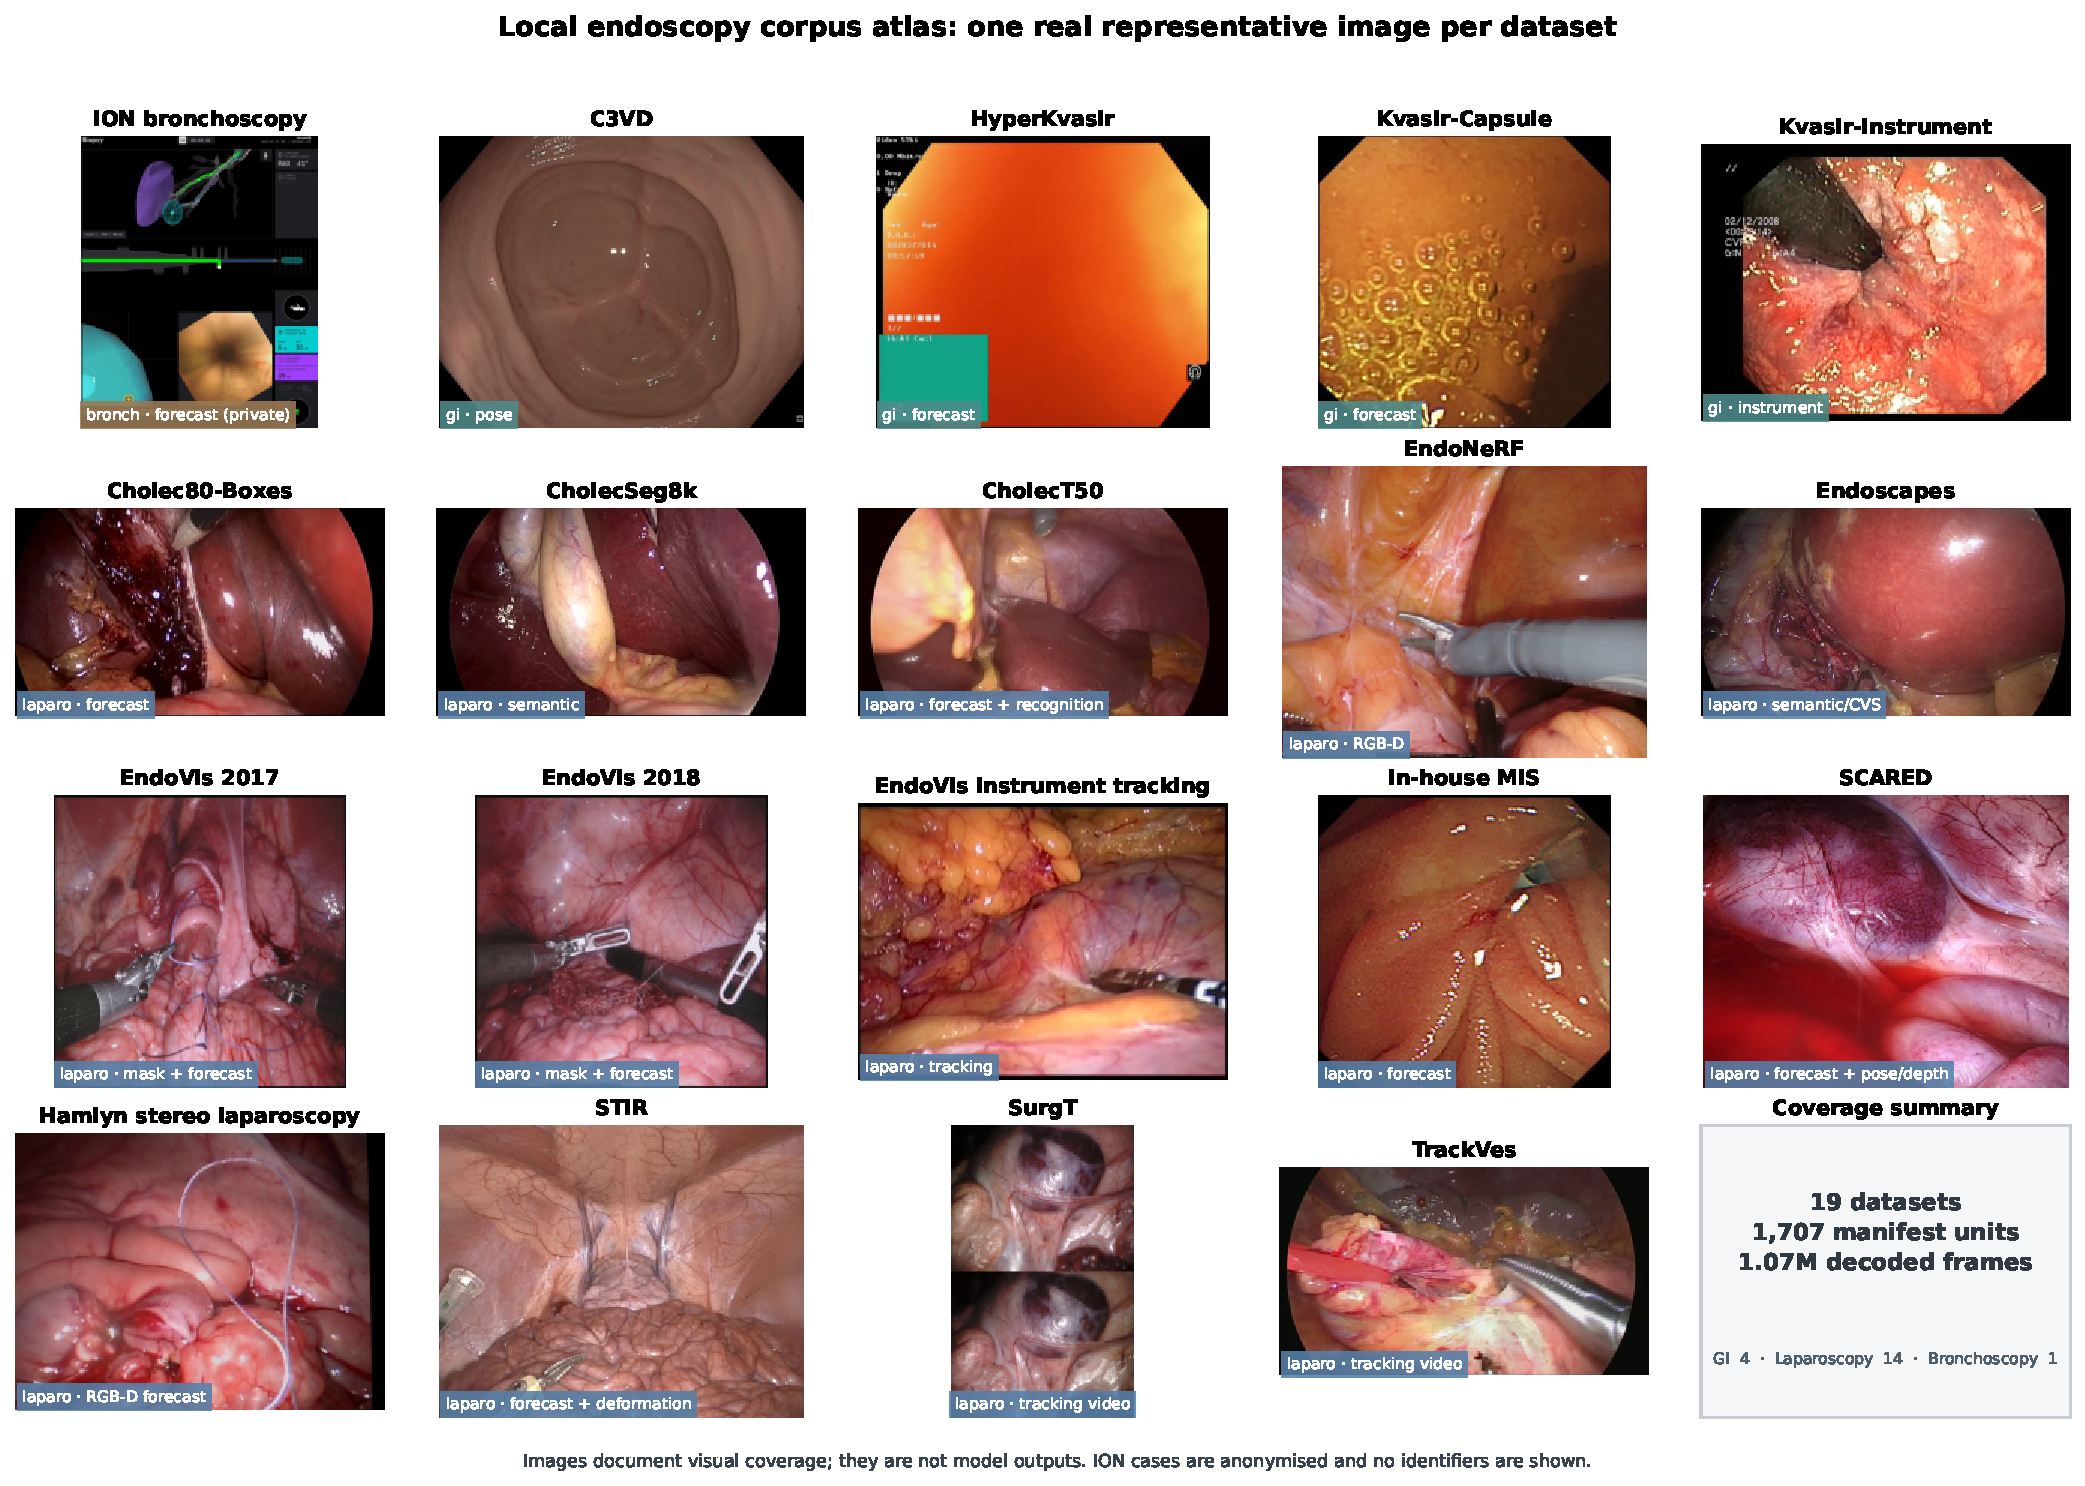
\includegraphics[width=\textwidth]{figure9_dataset_atlas.pdf}
\caption{Complete visual atlas of the 19 local datasets in
Table~\ref{tab:census}, with one real representative image per dataset.
The twentieth grid cell is an explicit coverage summary, not a missing dataset.
This figure documents corpus coverage rather than model output. It exposes the
large appearance shift between flexible GI, rigid laparoscopy and private
anonymised ION bronchoscopy, and the supervision shift from ordinary RGB to
pose, depth, mask and tracking corpora. Each cell is a real source frame
selected by a deterministic rule: image directories are scored at five fixed
temporal positions, whereas video-only assets use the decoded midpoint frame.
The source path, asset type and score are recorded with the figure. No patient
identifier is displayed.}
\label{fig:dataset-atlas}
\end{figure*}

\paragraph{Visual corpus audit}
Figure~\ref{fig:dataset-atlas} makes three properties hidden by aggregate frame
counts explicit. First, GI data span conventional colonoscopy, capsule imagery
and pose/depth-annotated colon-phantom C3VD, so ``GI'' is not a single
appearance distribution.
Second, laparoscopy ranges from standard cholecystectomy to stereo/RGB-D,
deformation and instrument-tracking views; these datasets provide complementary
supervision but are not interchangeable test sets. Third, ION bronchoscopy
contains both navigation-interface context and endoluminal imagery, motivating
explicit domain conditioning. The atlas is therefore evidence for domain
heterogeneity, not evidence of forecast accuracy.

\paragraph{Metrics}
The reported forecast score at maximum horizon $H$ averages cosine similarity
over all rollout steps $1{:}H$ and validation clips:
\begin{equation}
\mathrm{cos}_{1:H}
=
\frac{1}{|\mathcal{V}|H}
\sum_{v\in\mathcal{V}}\sum_{h=1}^{H}
\frac{
\langle \hat{\bar z}^{(v)}_{t+h},\, \bar z^{(v)}_{t+h}\rangle
}{
\|\hat{\bar z}^{(v)}_{t+h}\|_2\,\|\bar z^{(v)}_{t+h}\|_2
},
\label{eq:cos}
\end{equation}
where $\mathcal{V}$ is the video-level validation clip set. MSE uses the same
clip-and-step aggregation and additionally averages over the $D$ latent
coordinates. Thus ``$H{=}4$'' in quantitative tables means the cumulative mean
over steps 1--4; terminal-step retrieval figures are labelled separately.
Higher cosine and lower MSE are better.
Physical association is reported as a real-action win fraction and inverse
$R^2$. The oracle-goal retrieval proxy reports a window-level win fraction and
retrieved-pose translation reduction; for source pose $\mathbf T_a$ and target
pose $\mathbf T_b$, translation error is
$\|(\mathbf T_a^{-1}\mathbf T_b)_{1:3,4}\|_2$. It is not executed reach. We additionally
report bootstrap summaries, near-wall area under the receiver-operating
characteristic curve (AUC), Brier score, expected calibration error (ECE) and
conformal coverage. The documented physical checks were pose-delta $R^2>0.3$,
real-action preference $>80\%$, and near-wall AUC $\ge0.75$ on at least 500
transitions. Risk fails the AUC gate (0.523). The oracle-goal retrieval has no
navigation success criterion because no action is executed.
Recognition uses video-level linear-probe phase accuracy and instrument mean
average precision (mAP; mean $\pm$ standard deviation over 3 seeds).
Action grounding uses normalised mutual information (NMI) versus a random-id
baseline.

\paragraph{Baselines}
Dynamics: persistence, GRU and a custom Mamba-inspired gated recurrence. The historical parallel-query run is
archived rather than treated as a baseline because its Transformer encoder was
bypassed.
Representation: ImageNet ViT, DINOv2, VideoMAE, TimeSformer and ViViT are
evaluated only within their stated CholecT50 protocol; results from different
challenge and cross-validation splits are not combined.
Pixel contrast: next-frame CNN and conditional DDPM.
V-JEPA~2-AC and SurgRec-JEPA have no public endoscopic-planning checkpoints;
their papers are cited, but no numerical comparison is reported.

\paragraph{Statistics}
Paired bootstrap summaries are computed over the 750 validation clips for
effect-size precision. Because clips from a sequence are correlated, these are
descriptive clip-level intervals rather than independent sequence-level
significance tests; the video-level split and per-dataset decomposition bound
the scope of inference.

\paragraph{Implementation}
Single GPU; encoder cached once; AdamW as in Section~\ref{sec:method}.
Hyperparameters: hidden $512$, $8$ heads, $4$ layers, dropout $0.1$ and
history/horizon $4/4$. The optional dense path uses VICReg weight
$0.1$; headline pooled checkpoints do not activate it.
Legacy sensitivity files vary depth, width and learning rate, but they do not
jointly record cache identity, seed and the complete command. No quantitative
hyperparameter-robustness conclusion is drawn from them.

\subsection{Capability 1: forecasting scene evolution (latent forecast and data scale)}
\label{sec:rq1}

\begin{table}[t]
\centering
\caption{Video-level latent forecast averaged over steps 1--4
($H{=}4$; 6{,}000-clip training, bidirectional-encoder shared cache).
All models use the same 750-clip validation set.}
\label{tab:forecast}
\small
\begin{tabular}{lcc}
\toprule
Model & cos$_{1:4}$ & MSE$_{1:4}$ \\
\midrule
Persistence & 0.916 & 0.532 \\
Mamba-inspired gated recurrence & 0.971 & 0.180 \\
GRU dynamics & 0.974 & 0.161 \\
\textbf{Endo-HJEPA (causal L1)} & \textbf{0.978} & \textbf{0.139} \\
\bottomrule
\end{tabular}
\end{table}

Table~\ref{tab:forecast} and Figure~\ref{fig:forecast} are the headline forecast result.
Causal L1 exceeds persistence, the custom gated recurrence and GRU on the same 750-clip validation
set, with the lowest MSE.
The margin over GRU is small in absolute cosine: at $h{=}1$, the clip-level
paired difference is $0.00335$ (bootstrap 95\% interval
$[0.00300,0.00371]$); for the mean over steps 1--4, it is $0.00360$
($[0.00321,0.00398]$). These intervals quantify resampled clip variation and
do not establish independent sequence-level significance. The practical
effect should therefore be read with the per-dataset decomposition, rather
than from a small nominal $p$-value.
The valid comparison therefore supports a small advantage of causal L1 over
the recurrent baselines; it does not isolate causal masking from model size or
residual parameterisation.

The scale curve (Figure~\ref{fig:forecast}a) is monotonic from $500$ to $6{,}000$ clips ($0.962\to0.968\to0.972\to0.976\to0.978$); it overtakes the $6$k GRU ($0.974$) only from $4{,}000$ clips onward, so the causal Transformer needs moderate data before its advantage materialises.
Extending causal L1 to all $13{,}552$ pooled clips that the local corpus yields
gives cosine $0.978$ and MSE $0.135$ on a different validation cache
($n{=}1{,}631$). Because both the training and validation caches change, this
point cannot establish a scaling plateau or isolate the effect of additional
training clips.

As a lightweight sanity check rather than a generative-world-model SOTA
comparison, a next-frame CNN evaluated on 200 clips reaches $17.9$\,dB PSNR
against copy-last $29.6$\,dB; a conditional DDPM evaluated on 64 clips reaches
$4.9$\,dB against copy-last $30.4$\,dB
(Figure~\ref{fig:aux}a). These limited-budget baselines are consistent with,
but do not prove, the representation-prediction argument.

\begin{figure}[t]
\centering
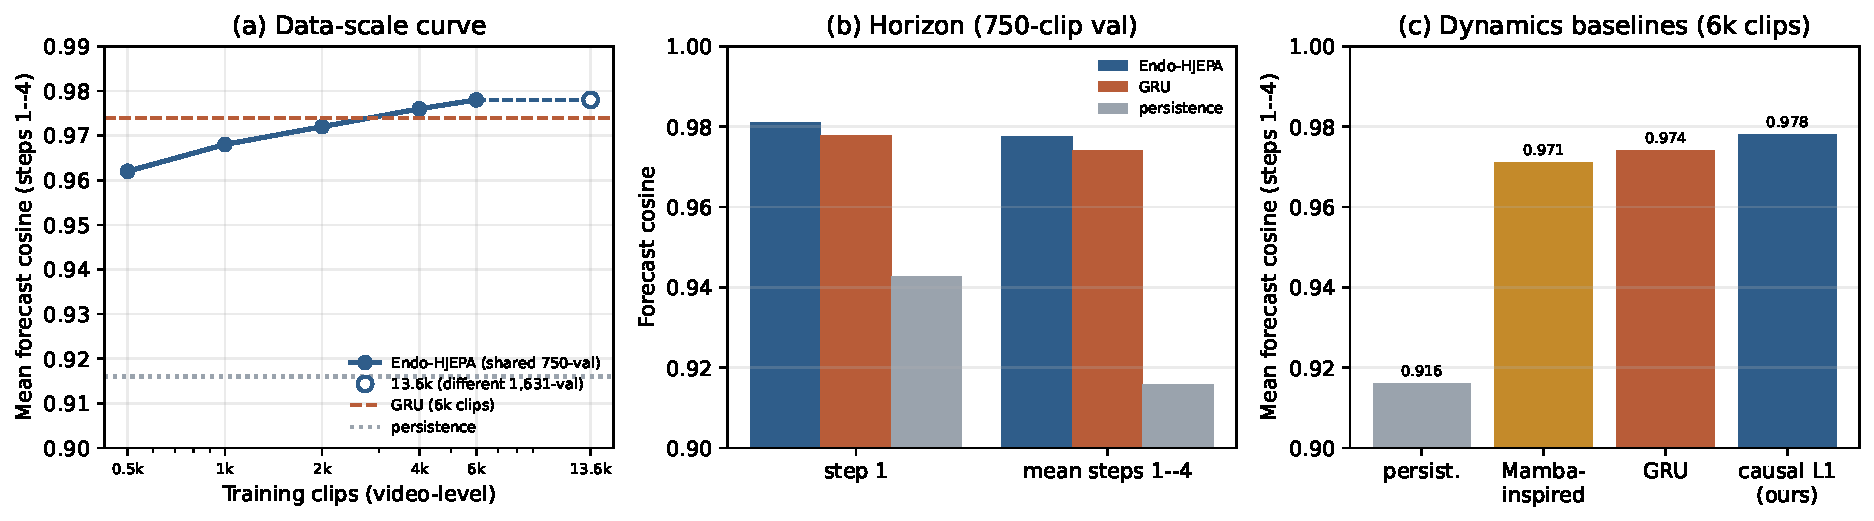
\includegraphics[width=\textwidth]{figure2_forecast.pdf}
\caption{(a)~Forecast cosine versus training clips on the bidirectional
encoder cache; the open 13,552-clip marker uses a different 1,631-clip
validation cache and is connected with a dashed line, whereas 500--6,000 share
750 validation clips. GRU and persistence are $6$k-clip references. A separate
past-only sensitivity audit (not plotted here) yields $0.9578$ versus $0.9102$
persistence and is not interchangeable with these headline points.
(b)~Step 1 and the cumulative mean over steps 1--4 on the shared 750-clip
validation set (Table~\ref{tab:forecast} reports the latter, 0.978).
(c)~Same $6$k-clip protocol as Table~\ref{tab:forecast}.}
\label{fig:forecast}
\end{figure}

\subsection{Action-conditioned association and oracle-retrieval diagnostics}
\label{sec:rq3}
A post-hoc audit found that the original L2/L3 predictor constructed, but
never executed, its Transformer encoder in the forward pass. Its outputs were
therefore not functions of history or candidate action. The earlier 98.0\% latent-reach and 92.8\% energy-ranking
values remain in the audit archive, are marked invalid, and are removed from all
claims. The corrected continuous implementation executes block-causal
attention; its executable tests in Section~\ref{sec:audit} verify history and
action sensitivity, future-action non-leakage, and gradients to the action
projection and encoder. Domain sensitivity is tested only for the separate
legacy domain-conditioned path.

The initial energy/risk analysis used a one-frame misalignment between v2
latent steps and SCARED depth labels and is therefore archived. After rebuilding labels
with the corrected window-end mapping ($30+4k$ native frames) and retraining
the three-member probabilistic model, audit AUC is only $0.523$ over 3,832
overlapping window-step predictions (958 windows $\times$ 4 steps; Brier
$0.246$, ECE $0.098$). The nominal 90\% split-conformal
interval covers 73.3\% of contacted-audit labels. Both discrimination and coverage are
insufficient, and AUC is below the documented $0.75$ gate.
Pre-correction risk AUCs are archived diagnostics and are not used as
evidence. Near-wall anticipation therefore remains unestablished, and the
reported CEM proxy does not activate a risk head or candidate-rejection
threshold.

The corrected v2 cache fixes stacked stereo input, bidirectional 64-frame
encoding, chunk resets and the original negative-protocol mismatch.
On the previously contacted SCARED audit partition, the deterministic batch-shuffled
comparison gives a real-action win fraction of \textbf{88.5\%}
($n{=}958$ windows across four sequences; real versus shuffled MSE 0.152 versus
0.223; inverse-action $R^2{=}0.546$). A separate bank of ten distinct
same-sequence negatives gives 92.2\% pair wins and 66.4\% all-negative wins.
The batch permutation is a derangement (no action remains paired with its own
window), and the fixed bank samples without replacement. These metrics use
distinct negative distributions and overlapping windows, so neither is
independent case-level confirmation. Four sequences are also insufficient for
a meaningful case-level confidence interval or hypothesis test.

C3VD actions use the implementation's OpenGL-to-OpenCV conversion. The
depth-warp diagnostic records target-depth consistency for that convention but
cannot independently select or validate its translation. The available
ten-trajectory action export predates the final derangement and
without-replacement negative evaluator; its percentages are archived and are
not used as external-generalisation evidence.

For the continuous candidate-search proxy, CEM samples normalised action
coordinates but receives the recorded terminal latent as an oracle target.
On 200 deterministically sampled windows from four SCARED audit sequences,
one open-loop search retrieves a strictly future recorded latent with lower
translation error than the current-state persistence pose in 97.5\% of windows
and a 43.8\% lower mean retrieval error. This high value is structurally
favoured because the candidate set excludes the current state and the target
latent is supplied by the recorded future. It is therefore a retrieval sanity
check, not a navigation success rate. The commanded endpoint has mean
translation error 2.85\,mm; no action is executed and no risk filter is active.
A slot-space ablation isolates the planner interface: factorised latent slots
retain action sensitivity on the development
validation partition (86.5\% fixed-bank pair win) but were not assessed on the
contacted audit partition or under the oracle-goal CEM proxy. We therefore
report the proxy only on the full pooled latent; near-wall risk does not meet
its evaluation gate and is unused in this proxy.

\begin{figure}[t]
\centering
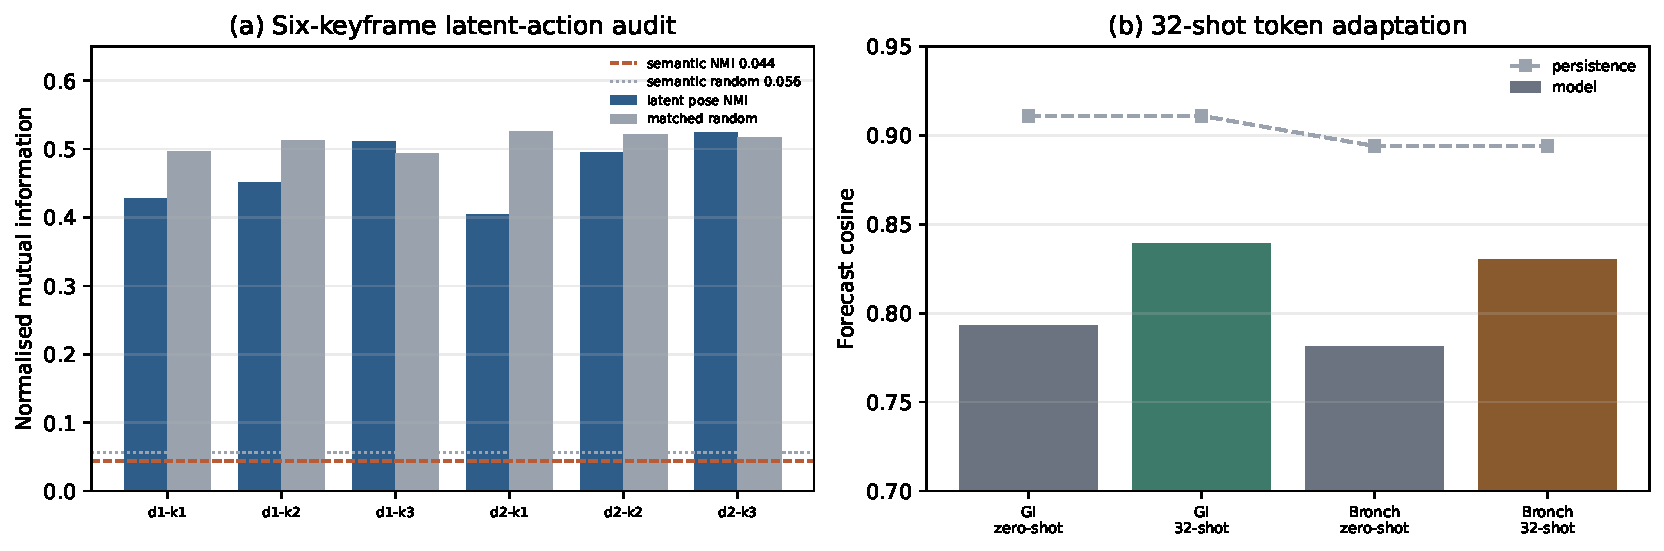
\includegraphics[width=\textwidth]{figure3_planning.pdf}
\caption{(a)~Latent-action audit on six SCARED keyframes: physical NMI is
plotted per keyframe against its matched random baseline, not as the midpoint
of a range; semantic NMI is a single corpus-level pair. Only two of six
keyframes exceed their matched random baseline. (b)~32-shot domain-token
adaptation from a laparoscopy-only model. Adaptation improves each target
domain but remains below persistence. The legacy 2,000-clip full-H-JEPA
forecast and discrete-MPC records are invalid because their encoder was not
executed and are excluded.}
\label{fig:planning}
\end{figure}

\begin{figure*}[t]
\centering
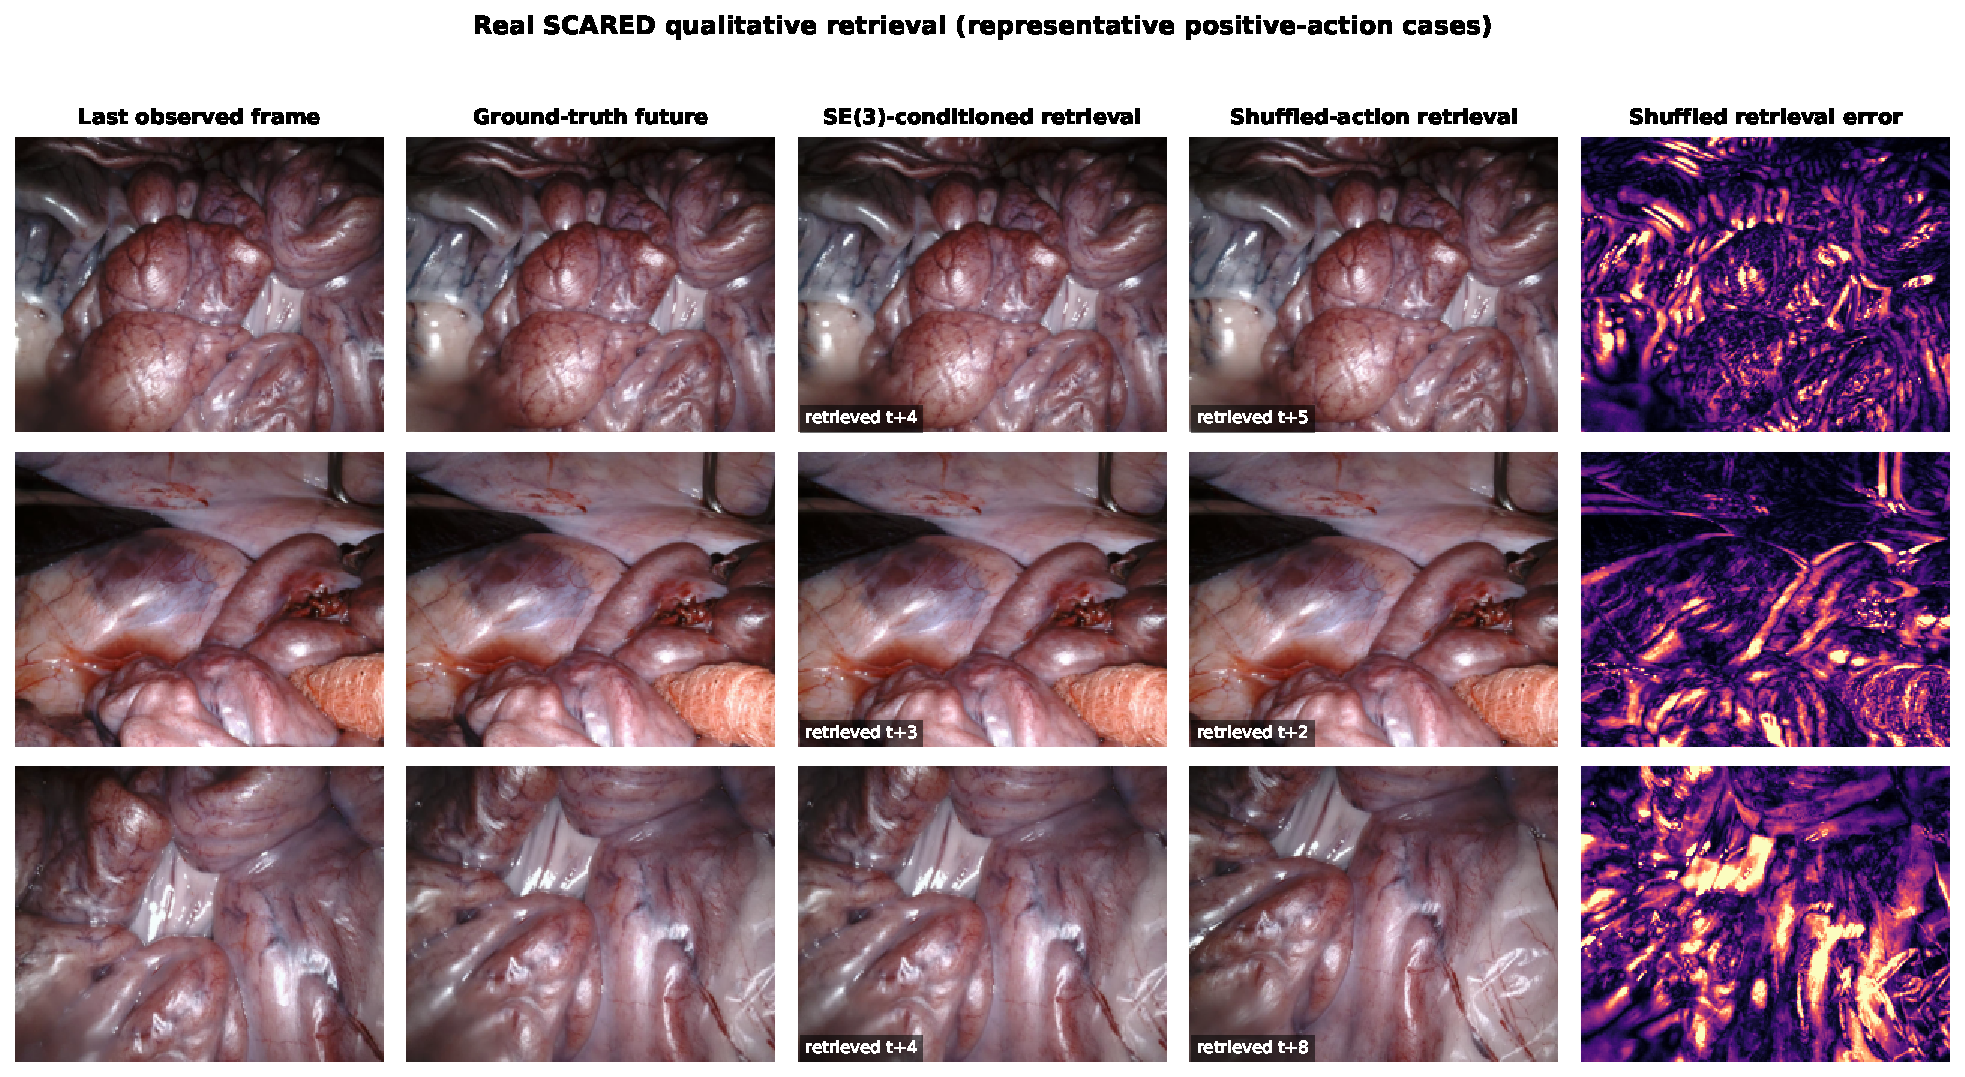
\includegraphics[width=\textwidth]{figure8_qualitative.pdf}
\caption{Real-frame qualitative results on SCARED audit sequences (v2
past-only, single-eye cache and model).
Because Endo-HJEPA predicts latent states and has no pixel decoder, visual
outputs are local nearest-neighbour \emph{retrievals}, not generated frames.
The candidate interval is the current latent through 16 later same-sequence
latents (truncated at sequence end), so recovery of the current frame is
allowed.
Consecutive SCARED frames are visually almost identical, so the informative
quantity is not the appearance of the retrieved frame but \emph{which} frame is
retrieved. Each row therefore reports the recovered temporal index and, on a
shared colour scale, the absolute image error of the real-action and the
deranged-action retrieval against the same ground-truth target. Rows are the
deterministic 25th/50th/75th percentile examples among cases where the
real-action prediction has both lower latent MSE and smaller temporal retrieval
error. The visual negatives use the same no-fixed-point, batch-size-32,
seed-0 derangement as the aggregate batch audit. The real action retrieves
$t{+}2$, $t{+}3$ and $t{+}2$, whereas the
deranged action retrieves $t{+}1$, $t{+}1$ and the current frame,
respectively. Real/deranged mean absolute image errors are $15.8/18.4$,
$19.7/37.9$ and $28.3/30.2$ intensity levels on the shared magma
colorbar (0--96). These panels illustrate
per-transition action use; the corresponding SCARED audit has an 88.5\%
batch-shuffled real-action win rate ($n{=}958$ overlapping windows from four
keyframe sequences), 92.2\% fixed-bank pair wins
and 66.4\% all-negative wins. These windows are audit-selected
descriptive evidence, not independent case-level inference; external C3VD
remains convention-specific.}
\label{fig:qualitative}
\end{figure*}

Figure~\ref{fig:qualitative} supplies image-level evidence while
preserving the distinction between latent prediction and pixel generation.
In the three deterministically selected positive-gain cases, the conditioned
latent retrieves a temporally closer index than its deranged-action counterpart
and incurs lower image error, although none recovers the exact four-step target.
Because the underlying frames change
slowly, recovered indices and error maps are reported in addition to the
near-identical retrieved frames. This remains
illustrative evidence; aggregate action-sensitivity values and their negative
protocols are reported above.
Figure~\ref{fig:rollout} shows the complementary four-step recorded-action
rollout on the same overlapping 958-window audit set: retrieval, not
navigation, and not an executed control sequence.

\begin{figure*}[t]
\centering
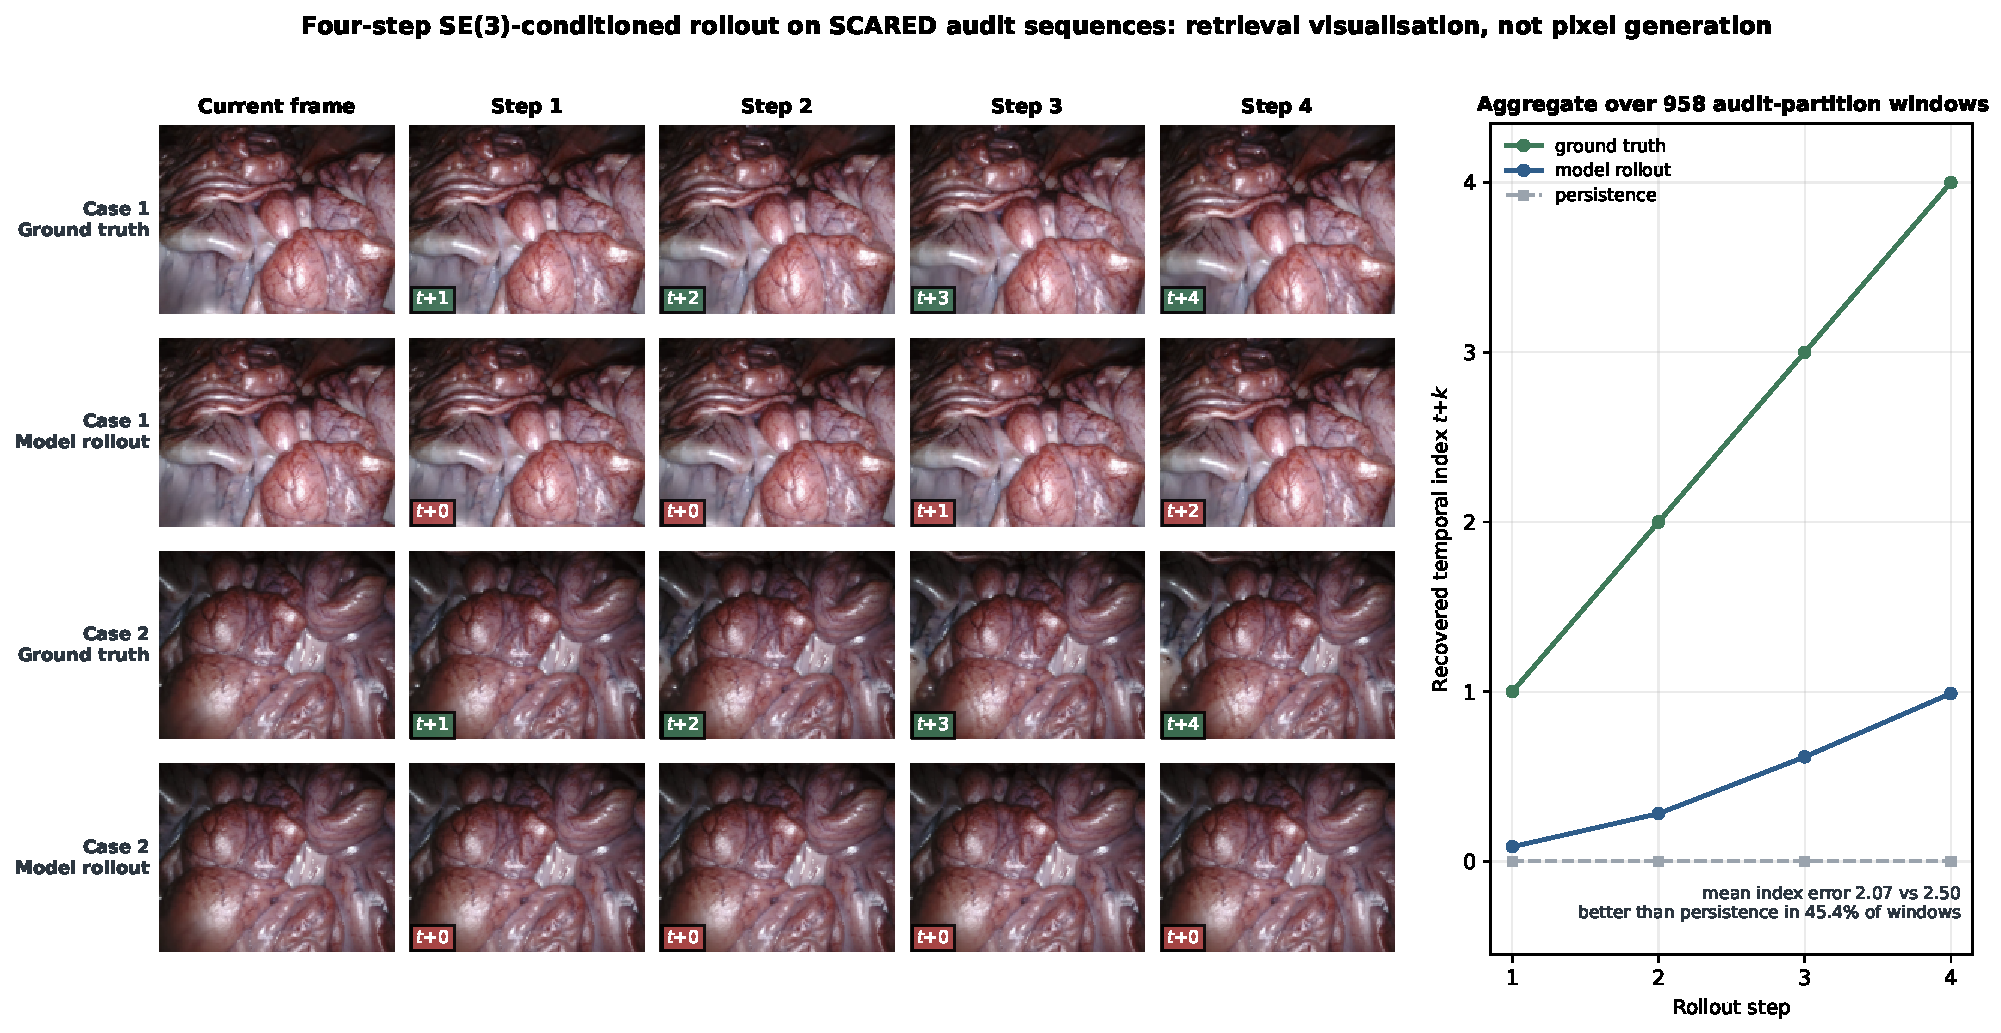
\includegraphics[width=\textwidth]{figure11_rollout_strip.pdf}
\caption{Four-step SE(3)-conditioned rollout on the training-excluded but
previously contacted SCARED audit partition (v2 model).
Each predicted latent is visualised by its nearest real frame within the same
sequence (retrieval, not generation), and every panel is annotated with the
temporal index it recovered: green when the rollout recovers the correct index,
red otherwise. Retrieval searches offsets 0--23 from the current latent,
truncated at sequence end. Cases are the lower-quartile and median rollout-index errors
over the audit partition and are illustrative rather than an estimate of a
typical independent case. The right panel aggregates all $958$ audit windows.
The mean recovered index increases with horizon but systematically lags the ground truth
($0.09, 0.28, 0.62, 0.99$ recovered indices against $1,2,3,4$), giving a mean
absolute index error of $2.07$ against $2.50$ for a persistence retrieval that
never leaves the current frame, and beating persistence in $45.4\%$ of windows.
These 958 windows overlap within four audit keyframe sequences; the
fractions are descriptive and are not a navigation or executed-control result.
This retrieval lag is consistent with under-predicted temporal displacement,
although nearest-neighbour matching cannot separate that effect from latent
ambiguity. Endo-HJEPA has no pixel decoder:
Section~\ref{sec:theory} shows pixel prediction is appearance-limited under
its stated idealised assumptions, and our lightweight pixel baselines are
consistent with that motivation (copy-last $29.6$\,dB versus $17.9$\,dB CNN and
$4.9$\,dB conditional DDPM; Figure~\ref{fig:aux}a).}
\label{fig:rollout}
\end{figure*}

\subsection{Limit A: cross-domain transfer}
\label{sec:rq4}
A laparoscopy-only model beats persistence in-domain ($0.922$ vs $0.850$) but falls \emph{below} persistence on zero-shot GI ($0.791$ vs $0.913$) and bronchoscopy ($0.776$ vs $0.893$).
Fine-tuning only the domain embedding on $32$ target clips recovers $+0.045$
on GI (evaluation $n{=}10$) and $+0.049$ on bronchoscopy
(evaluation $n{=}9$; Figure~\ref{fig:planning}b), but both remain below
persistence. This is partial recovery, not successful zero-shot adaptation.
The result does not compare unified and parameter-matched single-domain
training; it therefore motivates, but does not prove, a benefit from
multi-domain training or domain tokens.

\subsection{Limit B: unsupervised latent actions are not grounded (negative result)}
\label{sec:rq5}
Emergent latent actions are not physically grounded: SCARED pose NMI is
$0.41$--$0.52$ versus random $0.49$--$0.53$, and exceeds its matched random
baseline on only two of six keyframes; residual$\to$twist $R^2$ is negative.
They are also not semantically grounded (CholecT50 verb NMI $0.044$ versus
random $0.056$; probe accuracy $0.306$ versus majority-class $0.390$).
A codebook-level verb loss does not help.
Encoder-level verb supervision lifts residual$\to$verb NMI from chance $0.026$ to $0.056$: above chance, still weak.
Latent actions index visual change; they are neither discovered surgical
actions nor admissible control variables.

\subsection{Representation utility: downstream recognition probes}
\label{sec:rq6}

\begin{table}[t]
\centering
\caption{CholecT50 recommended official five-fold cross-validation
(50 videos; 10 test videos per fold; 3 probe seeds per fold).
Pooled linear probes use 800 clips; the dense multiple-instance learning
(MIL) probe uses 1{,}200 clips on
the same video folds and is therefore not an identical sampling protocol.
Values are mean $\pm$ standard deviation across the five fold means.}
\label{tab:downstream-cv}
\small
\begin{tabular}{lcc}
\toprule
Encoder & Phase accuracy & Instrument mAP \\
\midrule
V-JEPA 2 (frozen) & $0.683\pm0.040$ & $0.531\pm0.046$ \\
V-JEPA 2 (domain-adapted) & $0.679\pm0.038$ & $0.489\pm0.048$ \\
V-JEPA 2 (fine-tuned, dense MIL heads) & $0.711\pm0.031$ & $0.463\pm0.041$ \\
V-JEPA 2 (frozen, dense MIL probe) & $\mathbf{0.719\pm0.013}$ & $\mathbf{0.586\pm0.041}$ \\
\bottomrule
\end{tabular}
\end{table}

On the recommended research protocol, prediction-oriented adaptation improves
neither task. Frozen V-JEPA~2 is higher by $0.004$ phase accuracy and $0.043$
instrument mAP. This reverses the apparent instrument gain on the five-video
challenge split and shows why that smaller split must not be used for a
headline adaptation claim.
Probe \emph{capacity}, by contrast, matters: keeping the same frozen features
but replacing the pooled linear heads with a spatial MIL max-pool instrument
head and an attention-pooled phase head lifts phase to $0.719{\pm}0.013$ and
instrument mAP to $0.586{\pm}0.041$ on the same official five-fold video
split, using 1{,}200 clips rather than the 800-clip pooled-linear protocol.
Small instruments are spatially local, so mean-pooling may dilute the signal
needed for presence detection; the dense probe recovers part of the gap
without encoder supervision, but the mechanism is not isolated. End-to-end
fine-tuning of the last two blocks on the
same folds does not close the gap either. It degrades instrument mAP to
$0.463$, consistent with overfitting or loss of transferable features, though
the cause is not isolated. RDV reports instrument-component average precision
$\mathrm{AP}_{I}=0.894$ under its task-specific setup, rather than the simple
instrument-presence mAP used by our probe. The numerical gap may reflect label
definition, supervision scale, head capacity, architecture and representation
quality; the present experiments cannot attribute it to one factor.

\begin{table}[t]
\centering
\caption{CholecT50 official \emph{challenge-test} videos
(VID68, 70, 73--75), video-level linear probe, mean $\pm$ std over 3 seeds.
Each seed evaluates 80 test clips sampled from those five videos.
This is not the recommended five-fold cross-validation benchmark. We do not
claim uniform dominance.}
\label{tab:downstream}
\small
\begin{tabular}{lcc}
\toprule
Encoder & Phase acc & Instrument mAP \\
\midrule
ImageNet ViT (supervised) & $0.592\pm0.016$ & $0.430\pm0.003$ \\
DINOv2 (image SSL) & $0.658\pm0.016$ & $\mathbf{0.575\pm0.003}$ \\
VideoMAE (Kinetics SSL) & $0.558\pm0.012$ & $0.497\pm0.004$ \\
TimeSformer (video ViT) & $0.683\pm0.012$ & $0.490\pm0.010$ \\
ViViT (video ViT) & $0.692\pm0.024$ & $0.443\pm0.004$ \\
V-JEPA 2 (frozen) & $\mathbf{0.704\pm0.006}$ & $0.406\pm0.002$ \\
V-JEPA 2 (domain-adapted) & $0.688\pm0.057$ & $0.485\pm0.005$ \\
\bottomrule
\end{tabular}
\end{table}

\begin{figure}[t]
\centering
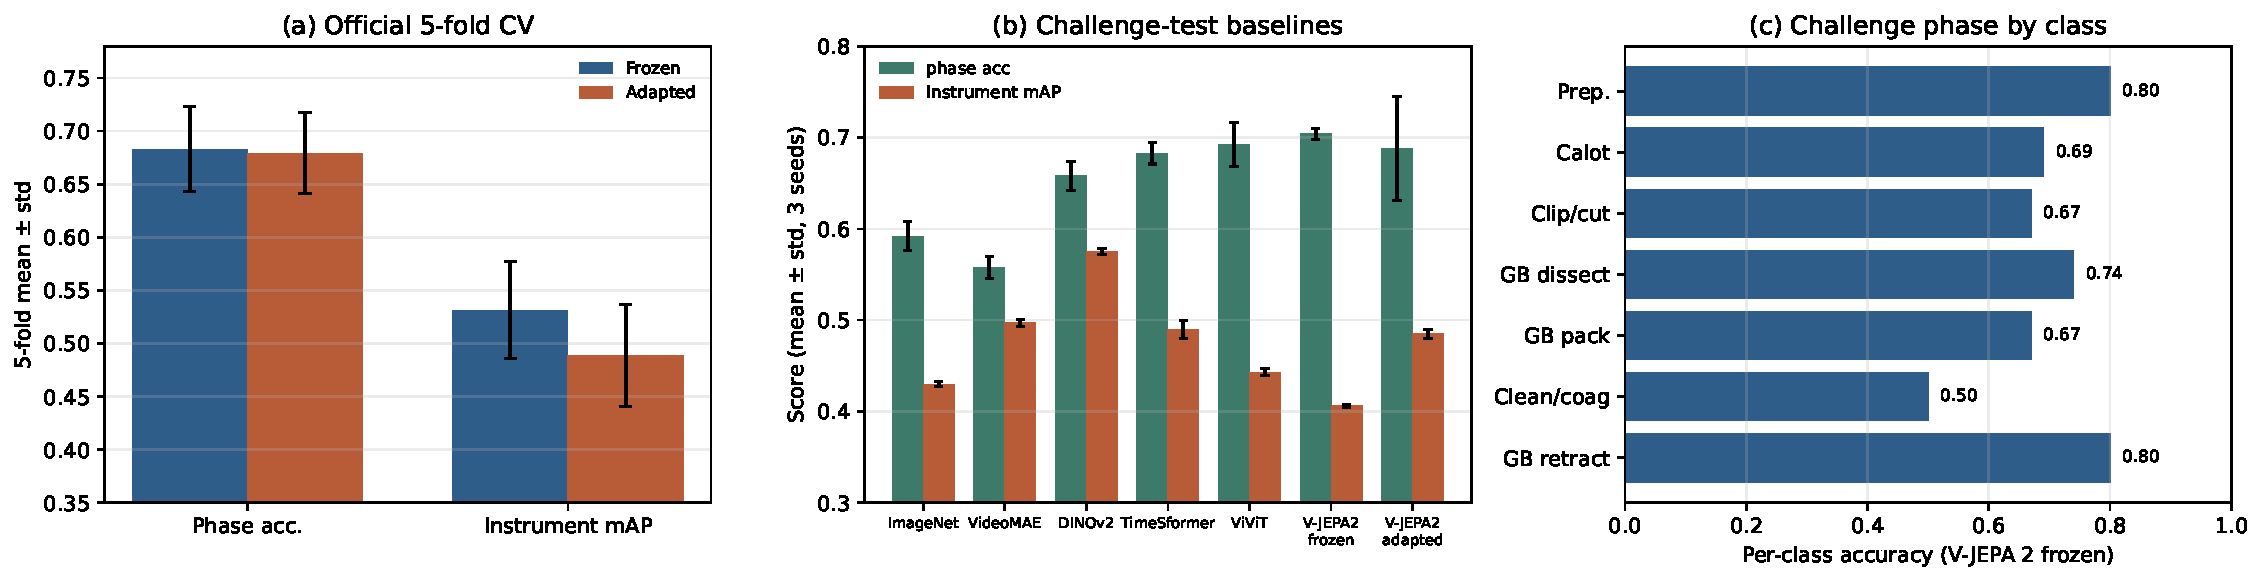
\includegraphics[width=\textwidth]{figure4_downstream.pdf}
\caption{(a)~Frozen-versus-adapted pooled linear probes from the recommended
official five-fold CV in Table~\ref{tab:downstream-cv} (800 clips); error bars
are standard deviations across fold means. The dense MIL row of that table is
not shown here because it uses 1{,}200 clips. (b)~Secondary challenge-test
backbone comparison matching Table~\ref{tab:downstream} (80 clips per seed on
five videos); error bars are 3-seed standard deviations.
(c)~Challenge-test per-class phase accuracy of frozen V-JEPA~2, corresponding
to Table~\ref{tab:perclass}.}
\label{fig:down}
\end{figure}

\begin{table}[t]
\centering
\caption{Challenge-test per-class phase accuracy for frozen V-JEPA~2
(official five-video split, 80 clips per seed). Values are three-seed means
$\pm$ standard deviations; class support is that of the official challenge
videos and is not re-estimated here. These class-level values
correspond to Figure~\ref{fig:down}c and are not five-fold CV estimates.}
\label{tab:perclass}
\small
\begin{tabular}{lcc}
\toprule
Phase & Accuracy & Seed std \\
\midrule
Preparation & 0.80 & 0.00 \\
Calot triangle dissection & 0.69 & 0.02 \\
Clipping \& cutting & 0.67 & 0.00 \\
Gallbladder dissection & 0.74 & 0.02 \\
Gallbladder packaging & 0.67 & 0.00 \\
Cleaning \& coagulation & 0.50 & 0.00 \\
Gallbladder retraction & 0.80 & 0.00 \\
\bottomrule
\end{tabular}
\end{table}

On the secondary challenge-test analysis (VID68, 70, 73--75; 80 clips per
seed), Figure~\ref{fig:down}b shows that frozen
V-JEPA~2 has the highest phase score among the evaluated local video backbones
($0.704$), while DINOv2
leads instrument presence ($0.575$). Adaptation shows a split-specific
instrument gain ($0.406\to0.485$), but Table~\ref{tab:downstream-cv} and
Figure~\ref{fig:down}a show that
it does not survive the recommended five-fold protocol. Figure~\ref{fig:down}c
and Table~\ref{tab:perclass} give the corresponding per-class phase breakdown.
This is an encoder-quality analysis, not a recognition-SOTA claim.
In the corrected patient-grouped STIR experiment, fine-tuning on 12 sampled
training sequences reduces the padded latent feature-set distance from 177.7 to 172.2
($-3.1\%$) over all eight sequences from two held-out patients
(Figure~\ref{fig:aux}c).

\paragraph{Literature and preprint context; non-comparability}
Table~\ref{tab:sota-context} states the comparison boundary explicitly.
The matched claim of this paper is limited to the baselines rerun on our
identical latent or challenge-test protocols. The cited task-specific reports
include both peer-reviewed articles and preprints; they use different labels,
supervision and splits and serve to identify the remaining gap rather than to
support a direct ranking.

\begin{table}[t]
\centering
\caption{Position relative to task-specific literature and preprints.
CV$=$cross-validation; SR$=$closed-loop success rate. Values in different
protocol columns must not be ranked directly.}
\label{tab:sota-context}
\footnotesize
\setlength{\tabcolsep}{3pt}
\begin{tabular}{L{0.18\textwidth}L{0.28\textwidth}L{0.25\textwidth}L{0.20\textwidth}}
\toprule
Task & Literature/preprint reference & Endo-HJEPA evidence & Valid conclusion \\
\midrule
CholecT50 instrument presence
& RDV $\mathrm{AP}_{I}=0.894{\pm}0.020$, official 5-fold CV~\cite{nwoye2022cholectsplit}
& Frozen V-JEPA~2 dense MIL $0.586{\pm}0.041$, same folds but 1,200-clip probe
& Related but non-identical labels/metrics and unequal supervision; no direct ranking \\
Cholec80 online phase
& SurgicalMamba $94.6{\pm}3.7\%$ accuracy under its reported protocol~\cite{surgicalmamba}
& Full Cholec80 is unavailable locally
& Required external benchmark remains open \\
Physical endoscope navigation
& EndoWAM $80.2\%$ SR on 96 phantom trials~\cite{endowam}
& 97.5\% forced-future oracle retrieval on 200 overlapping SCARED audit windows
& Structurally advantaged diagnostic; no executed navigation comparison \\
Surgical video generation
& SurgWM reports PSNR, structural similarity (SSIM) and Fr\'echet video distance (FVD)~\cite{svwm}
& No decoder; latent forecast cosine
& Orthogonal objectives and metrics \\
Latent endoscopic forecast
& No public benchmark matched to our frozen-encoder pooled-latent cosine/MSE protocol was identified as of 20 August 2026
& $0.978$ cosine versus matched persistence/GRU/custom gated recurrence
& Internal shared-cache comparison, not external SOTA \\
\bottomrule
\end{tabular}
\end{table}

\begin{figure}[t]
\centering
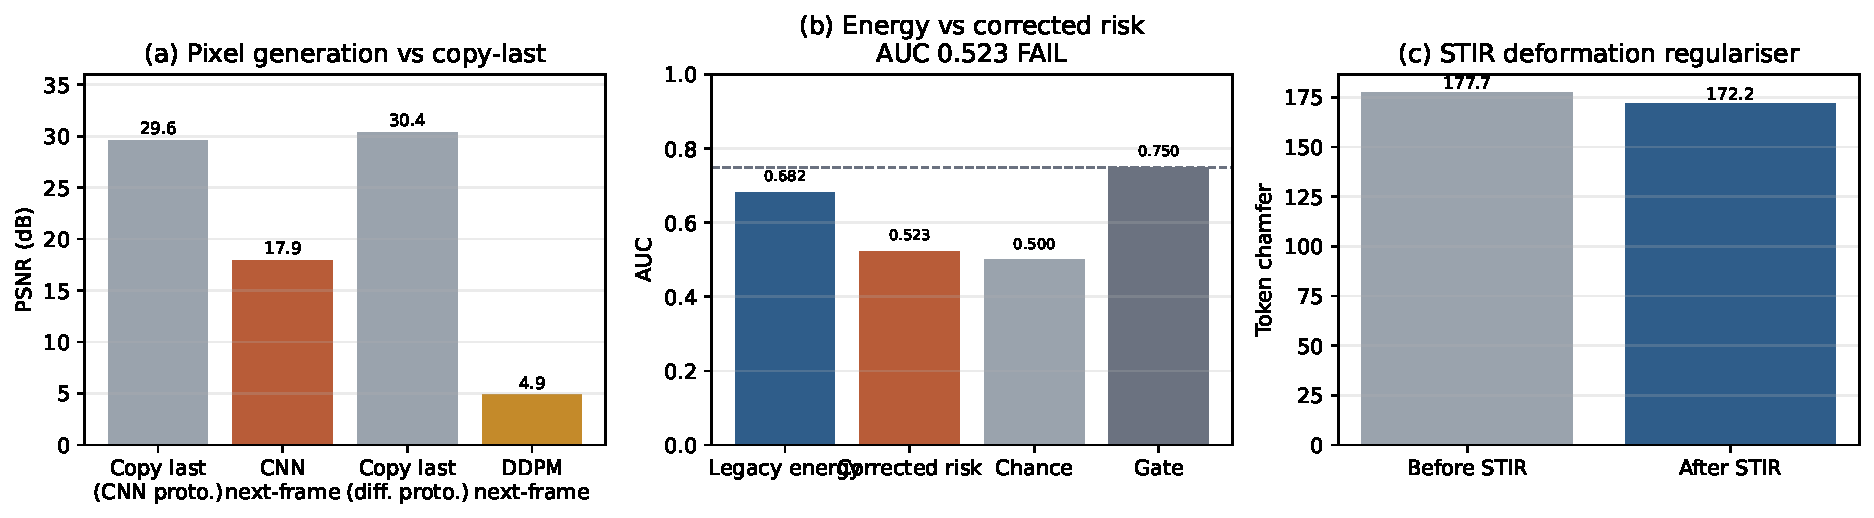
\includegraphics[width=\textwidth]{figure5_aux.pdf}
\caption{(a)~Lightweight pixel baselines (CNN: 200 clips; DDPM: 64 evaluation
clips) lose to copy-last; this is a sanity check, not a generative-model SOTA comparison.
(b)~Corrected-label risk head (AUC $0.523$ over 3{,}832 overlapping
window-step predictions), shown against chance and the documented $0.75$
gate; it is unused in the reported proxy.
(c)~STIR padded latent feature-set distance before/after the
regulariser~\eqref{eq:stir}, evaluated
on eight sequences from two patients excluded from fine-tuning.}
\label{fig:aux}
\end{figure}

\subsection{Per-dataset decomposition}
\label{sec:perds}
``Per-domain'' (three acquisition domains) hides dataset-level variation.
We reconstruct the same $750$-clip video-level val list used to build the $6{,}000$-clip cache (the domain-balanced sampler, seed $1$), attach dataset names, and evaluate the causal-L1 checkpoint.
Cache length and domain-ID order match the deterministic reconstruction
($n_{\mathrm{cache}}{=}n_{\mathrm{rebuilt}}{=}750$). The historical cache does
not store clip identifiers, so within-domain clip identity is assumed from the
replayed manifest, sampler and seed rather than independently verified.
Table~\ref{tab:perds} and Figure~\ref{fig:perds} report every dataset with $n{\ge}5$; SCARED and STIR appear with $n{=}1$ in the JSON and are omitted from the table.

\begin{table}[t]
\centering
\caption{Per-dataset latent forecast ($6{,}000$-clip causal L1, video-level
validation). Cosine values are means over steps 1--4; overall 0.978/0.916
matches Table~\ref{tab:forecast}.}
\label{tab:perds}
\small
\begin{tabular}{llrccc}
\toprule
Dataset & Domain & $n$ & cos & persist & $\Delta$ \\
\midrule
ION bronchoscopy & bronch & 250 & 0.988 & 0.918 & $+0.071$ \\
Kvasir-Capsule & gi & 206 & 0.978 & 0.941 & $+0.037$ \\
CholecT50 & laparo & 89 & 0.963 & 0.894 & $+0.069$ \\
Hamlyn stereo laparoscopy & laparo & 75 & 0.982 & 0.889 & $+0.093$ \\
Endoscapes & laparo & 72 & 0.961 & 0.893 & $+0.068$ \\
HyperKvasir & gi & 44 & 0.970 & 0.924 & $+0.046$ \\
EndoVis 2018 & laparo & 7 & 0.961 & 0.882 & $+0.079$ \\
EndoVis 2017 & laparo & 5 & 0.965 & 0.909 & $+0.056$ \\
\midrule
All val clips & --- & 750 & 0.978 & 0.916 & $+0.062$ \\
\bottomrule
\end{tabular}
\end{table}

\begin{figure}[t]
\centering
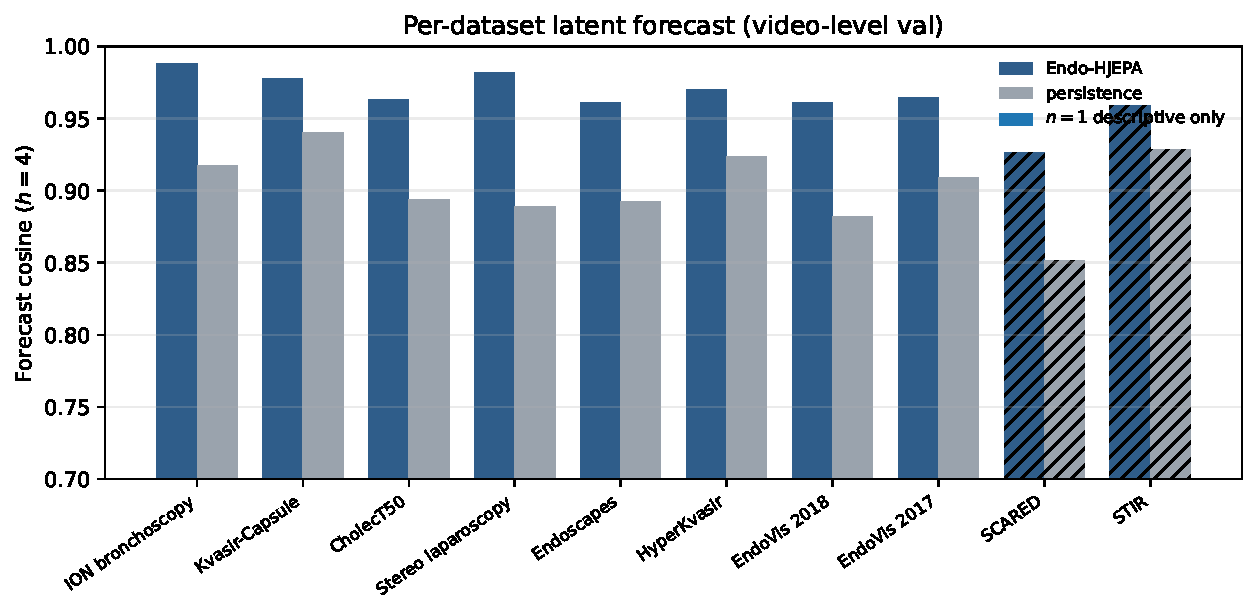
\includegraphics[width=\textwidth]{figure7_per_dataset.pdf}
\caption{Per-dataset forecast corresponding to Table~\ref{tab:perds}.
Hatch-marked $n{=}1$ rows (SCARED, STIR) are descriptive only and are not used
in the table. Among $n{\ge}5$ rows the largest margins are Hamlyn stereo laparoscopy
($+0.093$) and ION bronchoscopy ($+0.071$).}
\label{fig:perds}
\end{figure}

\begin{figure*}[p]
\centering
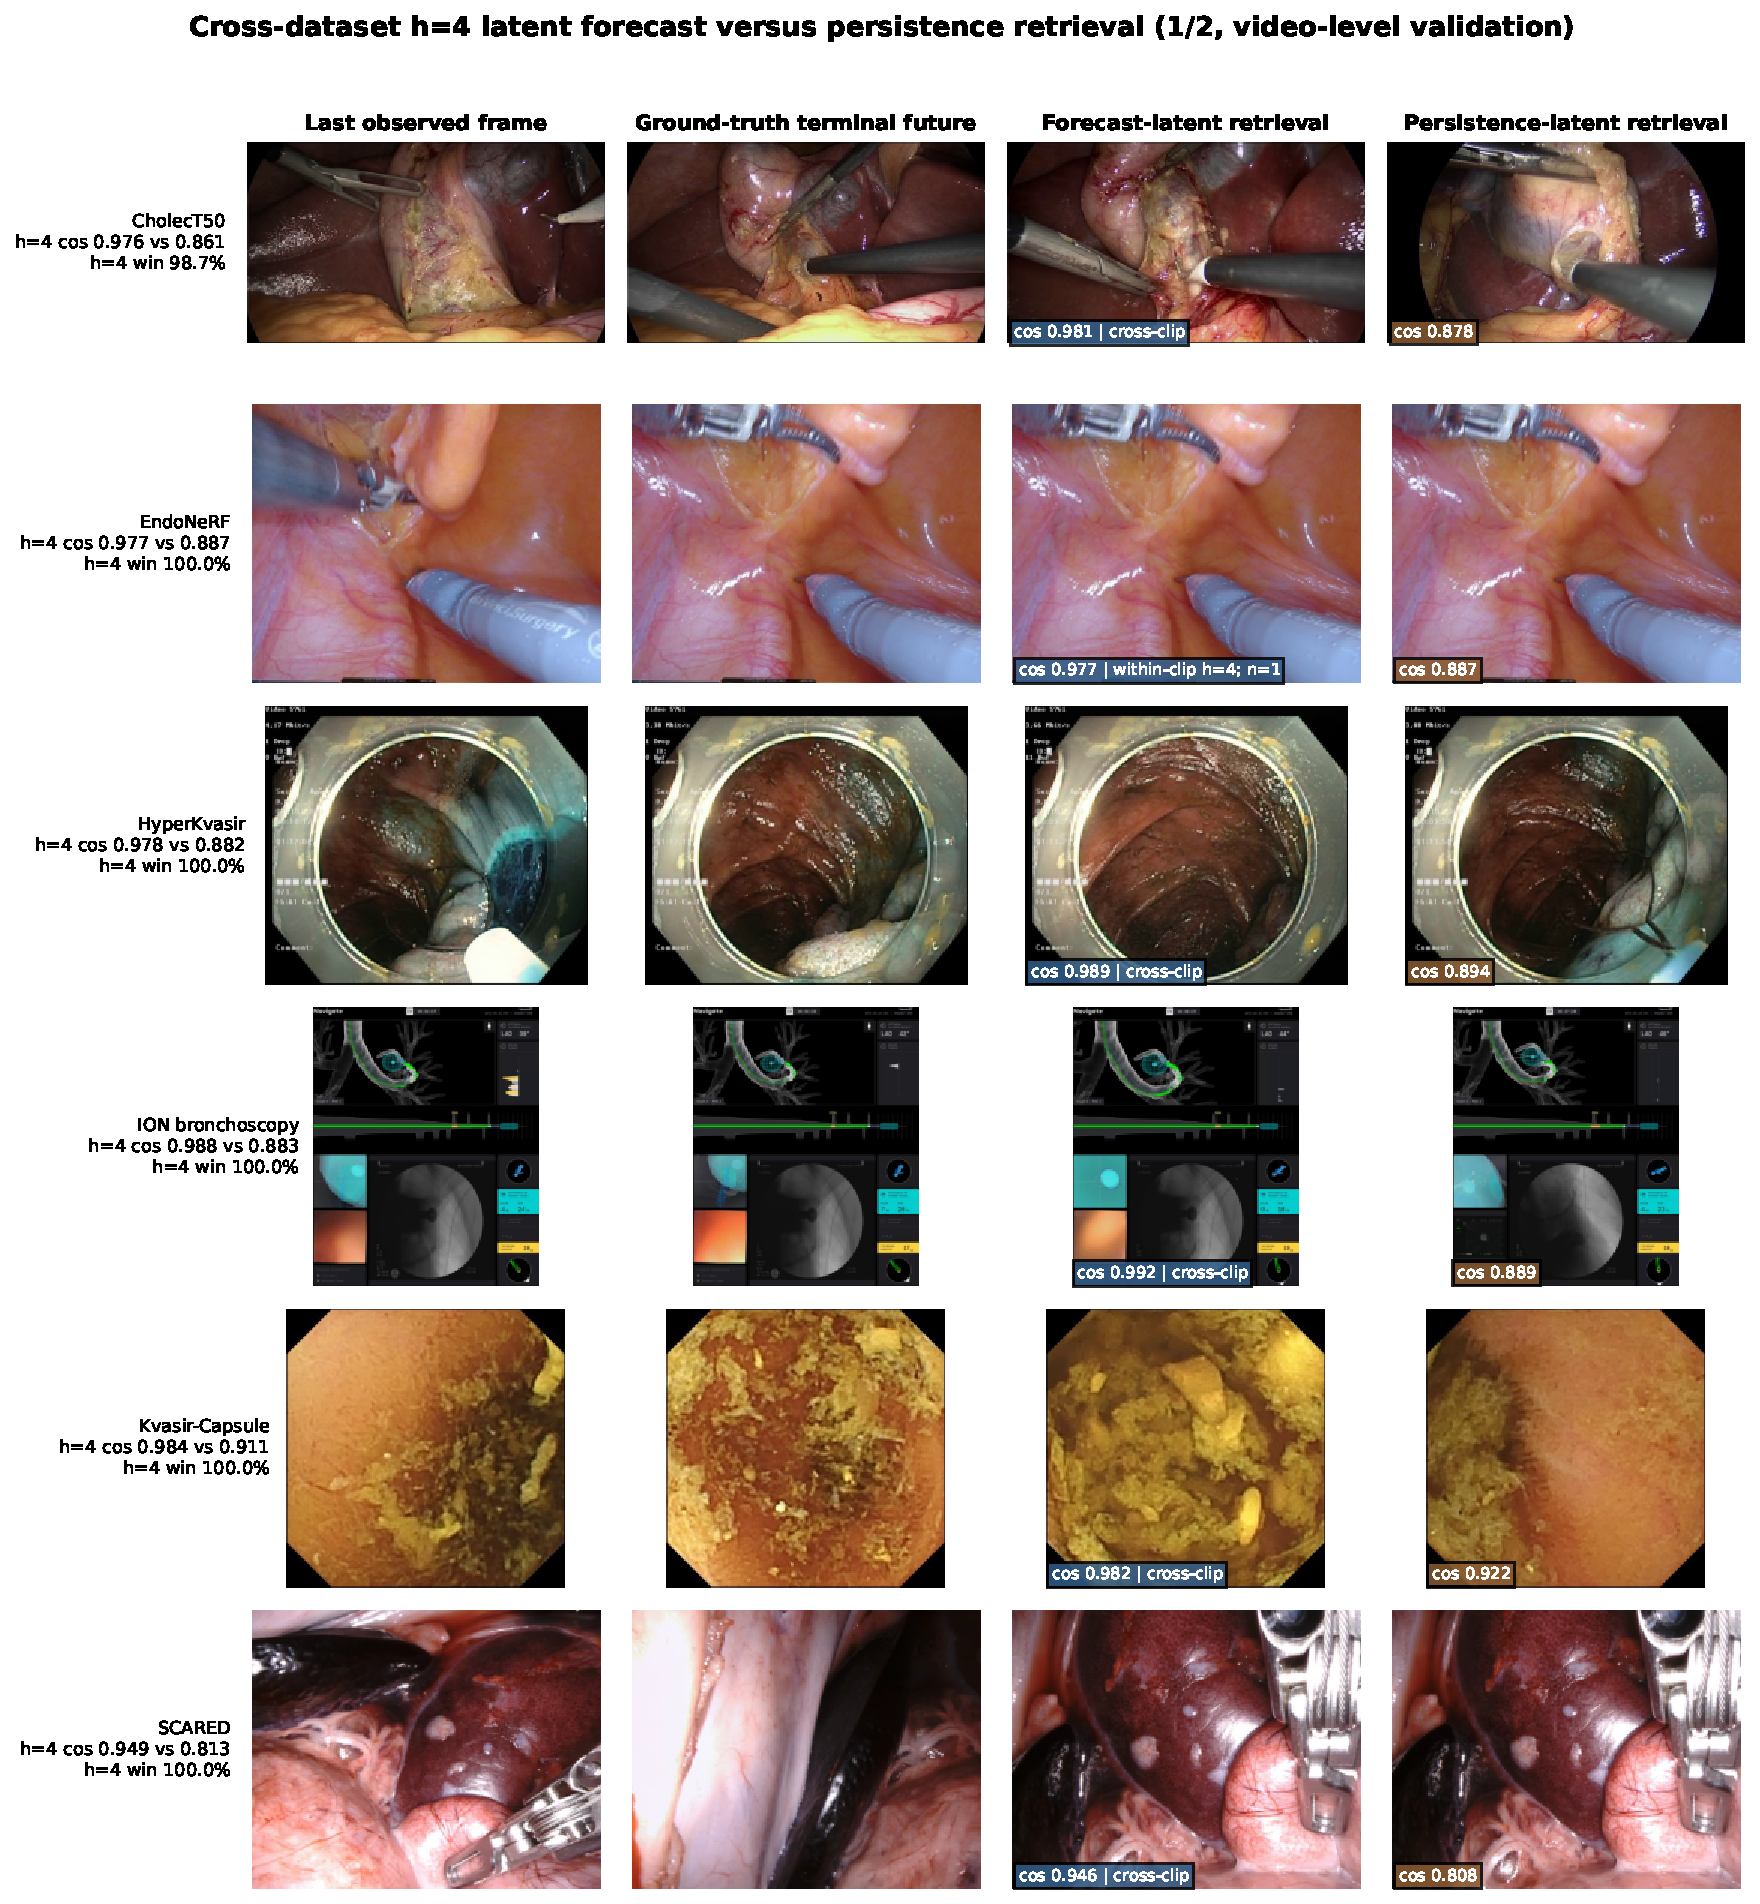
\includegraphics[width=0.94\textwidth]{figure10a_forecast_qualitative.pdf}
\caption{Cross-dataset visualisation (part 1 of 2) of the 13,552-clip causal-L1 checkpoint
on 1,631 video-level validation clips. All 11 datasets represented in that
cache are shown across this figure and Figure~\ref{fig:forecast-qualitative-all-b}.
Since the model has no pixel decoder, each predicted terminal
latent retrieves the nearest terminal frame from a \emph{different} validation
clip of the same dataset; EndoNeRF and STIR have $n=1$ and therefore use a
within-clip retrieval explicitly marked as such, in which case both retrieval
columns necessarily resolve to the same clip and only their cosines differ.
The last two columns apply that identical retrieval rule to two different
queries, the forecast latent and the last observed latent, so the figure shows
the same comparison that the aggregate numbers report rather than an
uninterpretable pixel difference between unrelated clips. Each retrieval panel
is annotated with the cosine of its query to the ground-truth terminal latent;
the forecast query is closer in every row shown.
Rows are deterministic median
positive-gain examples, not best cases. Left labels give the aggregate
dataset-level terminal-step cosine (model versus persistence) and terminal-step
transition win fraction;
retrieval visualises latent neighbourhoods and must not be read as
generated-pixel accuracy.}
\label{fig:forecast-qualitative-all}
\end{figure*}

\begin{figure*}[t]
\centering
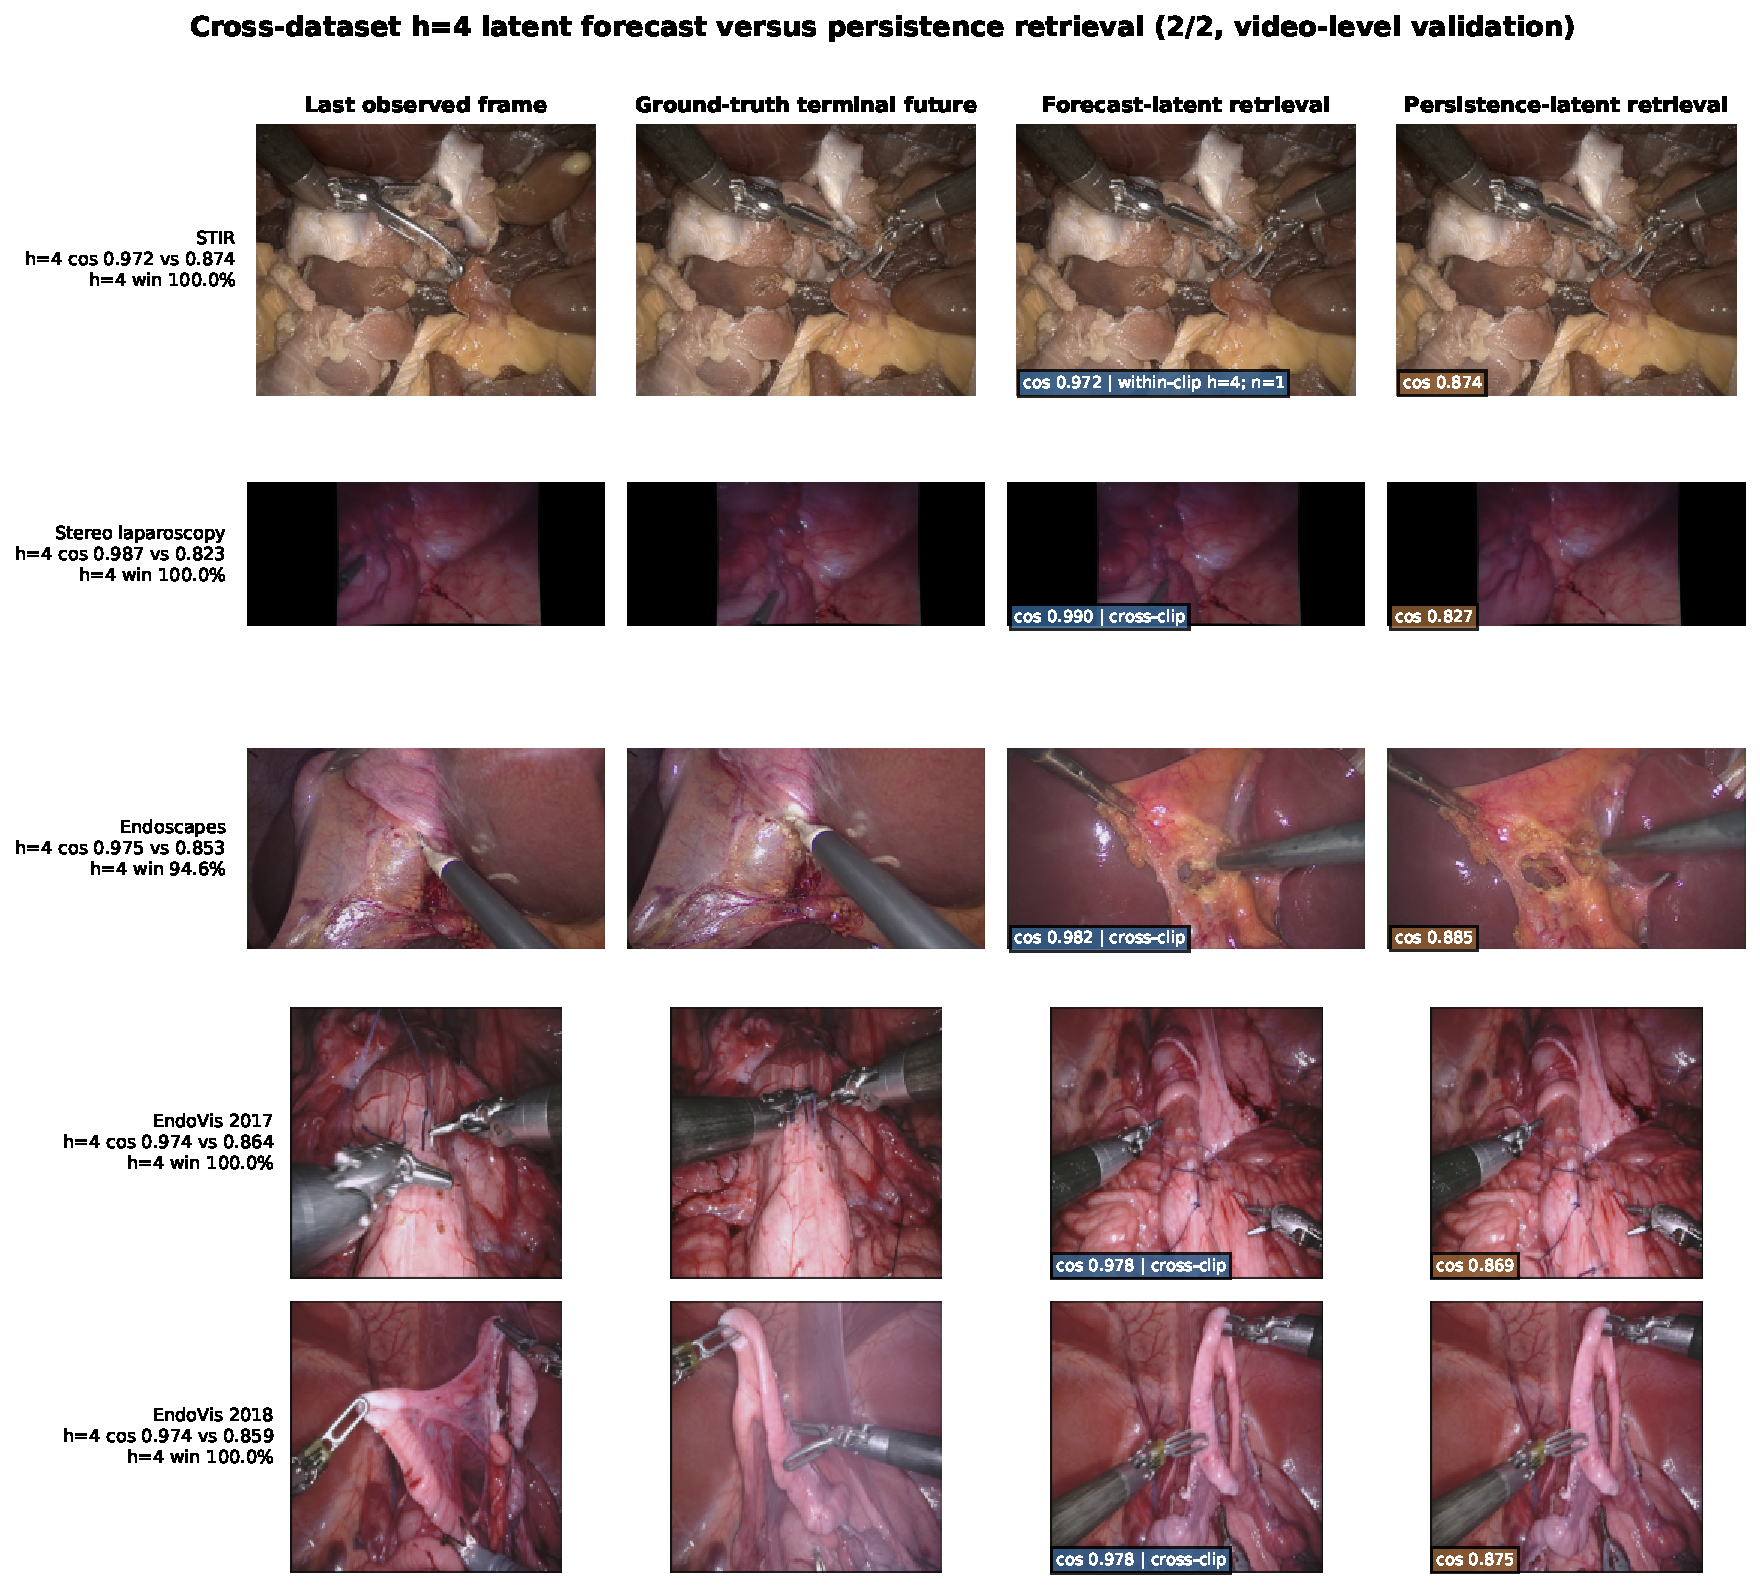
\includegraphics[width=\textwidth]{figure10b_forecast_qualitative.pdf}
\caption{Cross-dataset latent retrieval (part 2 of 2), under the identical
13{,}552-clip checkpoint, cache and selection rule of
Figure~\ref{fig:forecast-qualitative-all}.
Together the two panels cover every dataset represented in that cached
video-level validation split. The checkpoint, cache, split and selection rule
are recorded with the qualitative-protocol file.}
\label{fig:forecast-qualitative-all-b}
\end{figure*}

On the $6{,}000$-clip protocol of Table~\ref{tab:perds}, the unified model
beats persistence on every listed dataset with $n{\ge}5$ when averaged over
steps 1--4.
The largest margin is Hamlyn stereo laparoscopy ($+0.093$); ION bronchoscopy is next
($+0.071$). SCARED and STIR appear only as $n{=}1$ rows in the evaluation record
and are omitted from the table, so they cannot support a ranking.
Kvasir-Capsule has the highest persistence cosine ($0.941$)
and the smallest listed margin ($+0.037$): capsule motion is
slower, so copying the last token is already a good forecast.
This is the dataset-level reading of the $6$k claim. It does not establish
that unified training improves on
parameter-matched single-domain models. The larger 13{,}552-clip montage in
Figures~\ref{fig:forecast-qualitative-all} and
\ref{fig:forecast-qualitative-all-b} uses a different cache and must not be
mixed into Table~\ref{tab:perds}.

\paragraph{Cross-dataset qualitative conclusion}
The larger 13,552-clip cache in Figures~\ref{fig:forecast-qualitative-all}
and~\ref{fig:forecast-qualitative-all-b}
contains 11 datasets. At the terminal $h{=}4$, aggregate cosine exceeds
persistence for every row: the gains remain clear in ION bronchoscopy
(0.988 vs 0.883), Hamlyn stereo laparoscopy (0.987 vs 0.823), CholecT50
(0.976 vs 0.861), HyperKvasir (0.978 vs 0.882) and Kvasir-Capsule
(0.984 vs 0.911). Per-transition $h{=}4$ MSE win fractions are 94.6\%
for Endoscapes, 98.7\% for CholecT50 and 100\% for the remaining rows.
The latter must not be over-interpreted for EndoNeRF ($n=1$), STIR ($n=1$)
or SCARED ($n=4$). At the level of the individual examples shown, the forecast
query is closer to the ground-truth terminal latent than the persistence query
in all eleven rows, with per-example cosines such as $0.990$ against $0.827$
for Hamlyn stereo laparoscopy and $0.946$ against $0.808$ for SCARED, so the visual
comparison and the aggregate table tell the same story.
Cross-clip retrievals preserve broad anatomy, viewpoint and
tool context but can differ substantially in local tissue texture. Thus the
visual result supports predictable latent structure, not photorealistic future
synthesis.

Eight atlas datasets do not appear in this validation montage:
C3VD, Cholec80-Boxes, CholecSeg8k, Kvasir-Instrument,
EndoVis instrument tracking and the in-house MIS corpus have no validation clips under the
fixed manifest split; SurgT and TrackVes are video/tracking assets excluded
from the decoded-frame cache. Their images appear in
Figure~\ref{fig:dataset-atlas}; forecast outputs are omitted because these
datasets have no clips in the fixed validation split. The local C3VD corpus contributes no forecast-validation
clips. Its separate ten-trajectory external action manifest is reported only
in the action evaluation and therefore has no forecast output.

\FloatBarrier

\subsection{Model-comparison and ablation limits}
\label{sec:ablation}

Table~\ref{tab:forecast} provides the matched dynamics-model comparison. The
causal L1 model has the highest matched score, although the comparison does
not isolate its causal mask, residual anchor and architecture. A legacy
same-cache residual pair (0.768 without versus 0.900 with residual; persistence
0.886) lacks recorded train/validation sizes and seed, so it remains in the
ledger but is not used as an ablation claim. No full
L1{+}L2{+}L3{+}energy comparison is claimed: its legacy
2,000-clip record is invalid after the action-path audit and is excluded from
this table.
No hyperparameter-sensitivity conclusion is drawn because the legacy
depth/width/learning-rate note lacks a traceable run record.

\subsection{Reproducibility}
\label{sec:reproducibility}
Every experiment maps to a single documented entry point in the released
package: model training, per-dataset forecast evaluation, physical-action
cache construction, continuous-dynamics training with grouped
cross-validation, the oracle-goal retrieval proxy, the C3VD depth-warp
diagnostic, recognition probes, and risk calibration. Quantitative summary figures are generated from
the metric ledger or registered source report; cache-backed qualitative figures
recompute a fixed checkpoint, cache and selection rule. Captions identify the
applicable split and protocol; checkpoint and cache hashes for
Figures~\ref{fig:pipeline}, \ref{fig:qualitative} and \ref{fig:rollout} are
recorded in their provenance files. Encoder caches are
shared across matched ablations, and probe heads use fixed seeds.
Entry points, arguments and source reports for each table and figure are
documented with the released implementation. Large encoder caches and
checkpoints are not redistributed; experiments involving private ION or
in-house MIS video additionally require authorised data access.

\section{Discussion}

\subsection{Research significance and clinical path}
The reported outcomes are offline latent forecast and action-conditioned
association. They are relevant to three future research paths but have not
been evaluated for those applications. Forecasting could be linked to labelled
loss-of-view or time-to-contact endpoints; SE(3)-conditioned dynamics could be
tested for camera-handling assessment in a simulator; and the oracle-goal
retrieval diagnostic can be replaced by closed-loop phantom navigation.
Sharing representations across domains may also reduce data requirements for
bronchoscopy, but the present zero-shot results do not establish that benefit.
Clinical translation would require a pose/action-conditioned model, calibrated
time-to-contact or view-loss endpoints, prospective device-level testing, and
a human-factors study showing that warnings improve clinician performance
without increasing distraction. Latent cosine alone is not a clinical
endpoint.

\subsection{Evaluated contributions and scope}
The evaluated forecast configuration combines residual anchoring, causal L1
and domain tokens; current experiments do not isolate the contribution of any
one component. The physical contribution is a
correctness-audited pipeline that separates continuous SE(3) association,
negative protocols, risk-label timing and an oracle-goal CEM proxy. The latter
does not establish closed-loop control, active risk rejection or robot
execution. This distinction prevents a high latent similarity score from being
misrepresented as control.

\subsection{Failure analysis}
A small GRU is nearly competitive at $h{=}1$.
The original discrete action path failed an implementation sensitivity audit,
and unsupervised residual codes encode visual change, not steer commands;
metric SE(3) supervision and normalised-action CEM yield only an oracle-goal
retrieval diagnostic, not navigation. Corrected near-wall risk remains below
gate, and the legacy C3VD action export is excluded because it predates the
final negative evaluator.
Zero-shot GI/bronch transfer failure is consistent with substantial
cross-domain shift and motivates target-domain adaptation.
Together, these negative results identify action supervision and domain
adaptation as concrete next steps.

\subsection{Comparison to published and preprint world models}
Endo-HJEPA occupies a distinct design point: multi-domain representation
prediction without a pixel decoder, with action sensitivity tested against
pose measurements. The architecture includes a coarse L2 head, but the
reported forecast numbers are L1-only.
V-JEPA~2-AC is publicly released but action-conditioned for a Franka robot,
and SurgRec-JEPA is released as a pretrained representation backbone; neither provides an
endoscopic-planning checkpoint under our protocol. EndoWAM reports
physical phantom navigation without a public checkpoint, while SVWM and
CrossScope evaluate pixel generation, SurgFUTR evaluates labelled event
anticipation, and SurgWMBench evaluates instrument motion. We therefore report
selected task metrics in
Table~\ref{tab:sota-context} as non-comparable context rather than construct an
unmatched leaderboard.

\subsection{Limitations}
(i)~Training scale is far below SurgRec (${\sim}2{\times}10^8$ frames).
(ii)~Full Cholec80 depends on CAMMA access. The available C3VD action export
requires rerunning with the final negative evaluator before it can support an
external result.
(iii)~ION has no public telemetry or patient grouping key in the available
de-identified export; its sequence-level split cannot establish patient-level
non-overlap.
(iv)~Latent residual actions are not interpretable or controllable.
(v)~All planning is in silico. The SCARED action result is audit-selected,
with overlapping windows from four sequences rather than independent cases.
The CEM metric is a forced-future, single-shot oracle-goal retrieval
diagnostic, not offline replay or action execution. Risk is below gate after
label-aligned retraining (AUC 0.523).
(vi)~Val forecast is domain-balanced, so per-dataset $n$ is not proportional to corpus size; $n{=}1$ rows are omitted.
(vii)~Headline checkpoints use pooled latents; dense L1, VICReg,
specular/instrument weighting and STIR are optional extensions, not activated
together in those checkpoints.
(viii)~The original discrete-MPC values are invalid after the action-path
correctness audit and are excluded from evidence.
(ix)~One third of the 750-clip balanced forecast validation set comes from
private ION bronchoscopy, limiting independent reproduction; public-only and
external-site validation remain necessary.
(x)~The pooled forecast cache uses the encoder's bidirectional 16-frame
windows, so history tokens may carry limited future context within a window.
The 6,000-clip past-only audit obtains 0.9578 versus 0.9761 for a separately
recomputed bidirectional-cache comparator, while still exceeding its matched
persistence value (0.9102). This 0.9761 comparator is not the 0.9776
shared-cache headline value because the audit rebuilds the available history.
Because
the audit also changes the available encoder history, it is a sensitivity
analysis rather than an isolated estimate of future-attention inflation. The
physical-action cache (v2) already uses past-only look-back encoding.
(xi)~The principal forecast and action results are development-validation or
contacted-audit evidence. An untouched external test set is still required for
confirmatory performance claims.

\section{Conclusion}
Endo-HJEPA applies joint-embedding prediction to laparoscopic,
gastrointestinal and bronchoscopic video and separates latent forecast
evaluation from camera-motion conditioning. A coarse L2 head is implemented,
but the reported forecast comparison is L1-only. The past-only
causal-residual run surpasses its matched persistence baseline. On a
separate bidirectional validation cache, the forecaster is also higher than
persistence, GRU and the custom gated recurrence; this comparison is not an
independent test. After correcting single-eye input, past-only encoding
and negative sampling, the continuous SE(3) path gives 88.5\%
deranged-batch wins on 958 overlapping SCARED audit windows; a distinct
same-sequence bank gives 92.2\% pair wins and 66.4\% all-negative wins.
Corrected-label near-wall risk remains below gate (AUC 0.523). The
forced-future oracle retrieval is retained only as a diagnostic, while C3VD
action transfer, closed-loop navigation and risk calibration remain open. We
release the protocol, metric ledger and
figure generators; results requiring private ION data remain reproducible only
to authorised holders.

\section*{Declarations}
\textbf{Ethics approval and consent to participate.} Public datasets were used
under their original licences; the authors conducted no new animal
experiments. The private clinical component is a retrospective secondary
analysis of de-identified in-house laparoscopic and ION bronchoscopy videos.
Associated CT volumes were available under the same governance process but
were not used in the reported models or analyses. The responsible hospital
department de-identified the clinical data through its institutional review
process, and Dr.\ Nan Wei provided the resulting research data. Data access
and use were reviewed and authorised through the institutional
data-governance process of Henan Provincial People's Hospital. No prospective
enrolment, research-directed intervention or identifiable participant
information were involved, and the study complies with the Declaration of
Helsinki. The formal ethics approval or exemption identifier, decision date
and consent-waiver determination are not present in the available project
records and must be supplied by the responsible institution before submission.
\textbf{Competing interests.} None declared.
\textbf{Consent for publication.} Not applicable; no identifiable individual
data are presented.
\textbf{Funding.} This work was supported by the National Natural Science
Foundation of China (Grant No.\ 6240074117); the Henan University of Technology
Young Backbone Teachers Training Program (Grant No.\ 21421329); the Open
Project Program of the State Key Laboratory of Virtual Reality Technology and
Systems (Grant No.\ VRLAB2023C03); the Cultivation Project of Tuoxin Team in
Henan University of Technology (Grant No.\ 2024TXTD18); and the High-level
Talents Fund of Henan University of Technology (Grant Nos.\ 2022BS076 and
2022BS075).
The funders had no role in study design, data analysis, interpretation,
manuscript preparation or the decision to submit.
\section*{CRediT authorship contribution statement}
\textbf{Ranyang Li:} Conceptualization, Methodology, Investigation, Writing
-- original draft, Writing -- review \& editing,
Funding acquisition, Resources, Supervision.
\textbf{Nan Wei:} Conceptualization, Methodology, Investigation, Funding
acquisition.
\textbf{Zhipeng Lin:} Writing -- original draft.
\textbf{Wufeng Liu:} Methodology.
\textbf{Chao Fan:} Investigation.
\textbf{Xiaodong Guo:} Investigation, Resources, Writing -- review \& editing,
Supervision.
All authors reviewed and approved the final manuscript.
\textbf{Data/code availability.} All datasets are obtained from their original
sources subject to their licences and access restrictions. The implementation,
metric ledger, result records and figure generators are released at
\url{https://github.com/liranyang123456-commits/endohjepa}; independent
reproduction of ION- and in-house-MIS-derived values requires authorised
access to those private cohorts.
\textbf{Declaration of generative AI.} During manuscript preparation, the
authors used Cursor AI for language editing and code-review assistance. The
authors subsequently reviewed and edited the material and take full
responsibility for the content of the publication.

\bibliographystyle{elsarticle-num}
\bibliography{references}

\end{document}
